% Options for packages loaded elsewhere
\PassOptionsToPackage{unicode}{hyperref}
\PassOptionsToPackage{hyphens}{url}
\PassOptionsToPackage{dvipsnames,svgnames,x11names}{xcolor}
%
\documentclass[
  11pt,
]{article}
\usepackage{amsmath,amssymb}
\usepackage{setspace}
\usepackage{iftex}
\ifPDFTeX
  \usepackage[T1]{fontenc}
  \usepackage[utf8]{inputenc}
  \usepackage{textcomp} % provide euro and other symbols
\else % if luatex or xetex
  \usepackage{unicode-math} % this also loads fontspec
  \defaultfontfeatures{Scale=MatchLowercase}
  \defaultfontfeatures[\rmfamily]{Ligatures=TeX,Scale=1}
\fi
\usepackage{lmodern}
\ifPDFTeX\else
  % xetex/luatex font selection
  \setmainfont[]{TeX Gyre Termes}
\fi
% Use upquote if available, for straight quotes in verbatim environments
\IfFileExists{upquote.sty}{\usepackage{upquote}}{}
\IfFileExists{microtype.sty}{% use microtype if available
  \usepackage[]{microtype}
  \UseMicrotypeSet[protrusion]{basicmath} % disable protrusion for tt fonts
}{}
\makeatletter
\@ifundefined{KOMAClassName}{% if non-KOMA class
  \IfFileExists{parskip.sty}{%
    \usepackage{parskip}
  }{% else
    \setlength{\parindent}{0pt}
    \setlength{\parskip}{6pt plus 2pt minus 1pt}}
}{% if KOMA class
  \KOMAoptions{parskip=half}}
\makeatother
\usepackage{xcolor}
\usepackage[margin=2.2cm]{geometry}
\usepackage{longtable,booktabs,array}
\usepackage{calc} % for calculating minipage widths
% Correct order of tables after \paragraph or \subparagraph
\usepackage{etoolbox}
\makeatletter
\patchcmd\longtable{\par}{\if@noskipsec\mbox{}\fi\par}{}{}
\makeatother
% Allow footnotes in longtable head/foot
\IfFileExists{footnotehyper.sty}{\usepackage{footnotehyper}}{\usepackage{footnote}}
\makesavenoteenv{longtable}
\usepackage{graphicx}
\makeatletter
\def\maxwidth{\ifdim\Gin@nat@width>\linewidth\linewidth\else\Gin@nat@width\fi}
\def\maxheight{\ifdim\Gin@nat@height>\textheight\textheight\else\Gin@nat@height\fi}
\makeatother
% Scale images if necessary, so that they will not overflow the page
% margins by default, and it is still possible to overwrite the defaults
% using explicit options in \includegraphics[width, height, ...]{}
\setkeys{Gin}{width=\maxwidth,height=\maxheight,keepaspectratio}
% Set default figure placement to htbp
\makeatletter
\def\fps@figure{htbp}
\makeatother
\setlength{\emergencystretch}{3em} % prevent overfull lines
\providecommand{\tightlist}{%
  \setlength{\itemsep}{0pt}\setlength{\parskip}{0pt}}
\setcounter{secnumdepth}{-\maxdimen} % remove section numbering
\usepackage{etoolbox}
\AtBeginEnvironment{longtable}{\footnotesize}
\usepackage{caption}
\captionsetup{font=small,labelformat=empty}
\setlength{\tabcolsep}{4pt}
\usepackage{float}
\let\origfigure\figure
\let\endorigfigure\endfigure
\renewenvironment{figure}[1][]{\origfigure[H]}{\endorigfigure}
\ifLuaTeX
  \usepackage{selnolig}  % disable illegal ligatures
\fi
\IfFileExists{bookmark.sty}{\usepackage{bookmark}}{\usepackage{hyperref}}
\IfFileExists{xurl.sty}{\usepackage{xurl}}{} % add URL line breaks if available
\urlstyle{same}
\hypersetup{
  pdftitle={When Does Data Quality Help Human Deferral? Governance-Constrained Review Allocation in Knowledge-Based Decision Systems},
  colorlinks=true,
  linkcolor={Maroon},
  filecolor={Maroon},
  citecolor={Blue},
  urlcolor={Blue},
  pdfcreator={LaTeX via pandoc}}

\title{When Does Data Quality Help Human Deferral?
Governance-Constrained Review Allocation in Knowledge-Based Decision
Systems}
\author{}
\date{}

\begin{document}
\maketitle

\setstretch{1.25}
\textbf{Yeshwanth Reddy Kunam}\textsuperscript{a,*}

\textsuperscript{a} Doctor of Business Administration, Midwest
University, 851 Parr Road, Wentzville, MO 63385, United States

* Corresponding author. E-mail: yeshwanthkunam05@gmail.com

\emph{Revised author-review draft (October 2026). Not yet submitted or
peer reviewed.}

\hypertarget{highlights}{%
\section*{Highlights}\label{highlights}}
\addcontentsline{toc}{section}{Highlights}

\begin{itemize}
\tightlist
\item
  Exact sorting solves governance-constrained review allocation in both
  regimes.
\item
  Backlog depends on staffing, not on how mandatory cases are
  prioritised.
\item
  Learned deferral beat cost-aware heuristics only with thousands of
  review logs.
\item
  Quality inputs helped most when missingness was informative about
  outcomes.
\item
  Quality-triggered rules missed three-quarters of records with
  invisible defects.
\end{itemize}

\hypertarget{abstract}{%
\section*{Abstract}\label{abstract}}
\addcontentsline{toc}{section}{Abstract}

Organisations that automate decisions must decide which records a model
may decide alone, where scarce human review reduces expected loss, and
whether staff can absorb the review demand that governance rules make
compulsory. We study these choices in a knowledge-based routing system
combining a calibrated predictor, a data-quality rule base, a two-head
loss estimator that learns from incomplete review logs, and an allocator
that enforces review capacity and holds mandatory cases it cannot serve.
Sorting solves this governance-constrained allocation exactly in
feasible and overloaded regimes, and in a multi-period system the
backlog does not depend on how mandatory cases are prioritised. We
compare the system with published learning-to-defer surrogates,
differential triage and cost-aware heuristics under matched information,
rules, costs and capacity. The evaluation spans four credit datasets
(one with natural missingness), nine data-quality conditions including
defects invisible to validation checks, and five simulated reviewer
models, over 20 corrected repeated splits. Pooled, the proposed router
was the best learning-based method but 1.2\% costlier than Chow's
cost-risk rule. Learned routing overtook that rule only with roughly
1,800 or more training records, and with 6,000 it beat every comparator
on all splits. Quality information reduced cost mainly when missingness
was informative about outcomes (1.2--3.5\%), by improving estimates of
automated rather than reviewer error. In a 40-day simulation with a
deterioration episode, staffing determined backlog and service
completion far more than routing did. Quality-triggered rules blocked
most visibly degraded records but missed three-quarters of records with
invisible defects.

\textbf{Keywords:} Knowledge-based systems; Learning to defer; Data
quality; AI governance; Human--AI collaboration; Review capacity;
Managerial decision-making

\hypertarget{introduction}{%
\section{1. Introduction}\label{introduction}}

Organizations that automate operational decisions with machine-learning
models rarely automate everything. Credit, claims, compliance and
service-eligibility decisions are typically routed through a hybrid
process in which a model decides routine records and human reviewers
examine the remainder. AI-governance frameworks describe this division
of labour in terms of accountability, data controls and human oversight
{[}1--4{]}, and recent regulation makes human oversight an explicit
obligation for high-risk uses such as creditworthiness assessment
{[}5{]}. Requiring oversight, however, does not establish that oversight
is effective {[}6{]}. Managers still have to decide which records may be
automated, where scarce review effort reduces expected loss, and whether
staffing can absorb the review demand that governance rules make
compulsory.

Two research streams address parts of this problem. Learning to reject
and learning to defer (L2D) decide when a model should abstain or pass a
case to a human, trading model error against the cost or error of
deferral {[}7--12{]}. Algorithmic triage estimates human and model error
separately and automates the cases where the model is relatively
stronger {[}13, 14{]}, and recent work adds expert workload constraints
{[}15{]} or limited expert predictions {[}16{]}. In parallel,
data-management research treats completeness, validity and timeliness as
measurable properties of the inputs a model receives {[}17--19{]}.
Governance practice links the two: input-validation rules and model-risk
controls often require that records failing quality checks be reviewed
rather than automated {[}20{]}.

What is less well understood is how these elements interact when data
quality deteriorates. Mandatory-review rules triggered by quality checks
increase review demand precisely when review capacity is fixed; records
that cannot be reviewed are neither automated nor resolved; and a
quality signal that is informative about model error may or may not be
informative about reviewer error. Existing deferral studies typically
evaluate accuracy--coverage trade-offs with no compulsory review and no
unresolved cases, and data-quality studies rarely evaluate the
downstream allocation of human effort. An earlier draft of the present
study proposed a compact quality-conditioned gain model with two quality
rules and reported that, under a reviewer whose errors were simulated
from the same quality signals given to the router, the quality-aware
policy changed expected cost by only about 0.2\% relative to a
feature-aware comparator, with an interval that crossed zero. That
result raised three questions this revision is designed to answer:
whether the proposed method adds anything beyond published deferral
algorithms, whether its apparent value depended on a reviewer simulation
that favoured its own representation, and under which conditions
observable quality information is useful at all.

This paper therefore asks:

\begin{quote}
\textbf{RQ.} Under what data-quality and review-capacity conditions does
quality-aware deferral improve decision cost and service completion
while satisfying explicit governance rules?
\end{quote}

We study the question with a knowledge-based routing system consisting
of a calibrated predictor, a two-rule quality knowledge base, a two-head
loss estimator and an exact capacity-constrained allocator. The
contributions are as follows.

\begin{enumerate}
\def\labelenumi{\arabic{enumi}.}
\tightlist
\item
  \textbf{A governance-constrained allocation problem and its exact
  solution.} We formalise routing with automation, review and hold
  actions under a review budget, mandatory-review rules and a
  service-first constraint. We show that sorting solves the estimated
  problem exactly in both the feasible and the overloaded regime
  (Proposition 1). The overloaded case corrects the earlier draft, which
  ranked mandatory records by estimated gain even though automation loss
  is irrelevant for records that cannot be automated. We also show that,
  in a multi-period system, backlog size, workload and waiting cost do
  not depend on how mandatory records are prioritised (Proposition 2),
  which separates staffing decisions from prioritisation decisions.
\item
  \textbf{A two-head estimator that learns from incomplete review logs.}
  Expected review benefit is decomposed into an automation-loss head
  trained on all labelled records and a reviewer-loss head trained only
  on records with a logged review. This follows the triage logic of
  Raghu et al.~{[}13{]} but is tied to the allocation problem above and
  uses the reviewer-loss head directly for overload ordering.
\item
  \textbf{A matched benchmark against published deferral methods.} We
  compare the system with the cost-sensitive cross-entropy surrogate of
  Mozannar and Sontag {[}10{]}, the one-vs-all surrogate of Verma and
  Nalisnick {[}11{]}, differential triage {[}13{]} and Chow-type
  cost-risk rejection {[}7{]}. All methods receive the same information,
  rules, costs and capacity and are trained on noisy, incomplete review
  logs rather than on expected reviewer losses.
\item
  \textbf{A conditions analysis rather than a superiority claim.} Five
  reviewer models, four of whose errors do not depend on the router's
  quality signals and two of which err on information the router cannot
  observe, are crossed with two families of data defects: defects
  visible to completeness and range checks, and domain-valid defects
  (informative missingness, stale records and mis-keyed codes) that such
  checks largely miss. We add an external dataset with naturally
  occurring missingness. We report where quality information helps,
  where it does not and where it hurts, and how much review history a
  learned router needs before it beats a cost-aware heuristic. We also
  report managerial outcomes: review workload, backlog, waiting time,
  service-level attainment, override rate and cost per completed case.
\end{enumerate}

Section 2 reviews related work. Section 3 formulates the problem and the
method. Section 4 describes the experimental design and prespecified
hypotheses. Section 5 reports results, Section 6 discusses implications,
and Section 7 sets out limitations.

\hypertarget{related-work}{%
\section{2. Related work}\label{related-work}}

\hypertarget{rejection-deferral-and-triage}{%
\subsection{2.1. Rejection, deferral and
triage}\label{rejection-deferral-and-triage}}

Chow's rule rejects an input when the expected loss of the best decision
exceeds a fixed rejection cost {[}7{]}; modern variants learn the
rejector jointly with the classifier {[}8, 21{]} or wrap black-box
models {[}22{]}. Learning to defer replaces the constant rejection cost
with the loss of a specific human decision maker. Madras et al.~{[}9{]}
introduced the setting; Mozannar and Sontag {[}10{]} gave a consistent
cost-sensitive surrogate; Verma and Nalisnick {[}11{]} proposed a
one-vs-all surrogate with calibrated deferral probabilities; and later
work studied multiple experts {[}23, 24{]}, underfitting {[}25{]}, exact
mixed-integer formulations {[}12{]} and human--AI dependence {[}26{]}.
Triage methods estimate human and algorithmic error separately and rank
cases by their difference {[}13{]}, or learn the model and triage policy
jointly {[}14{]}. Several studies relax the assumption of complete
expert data: Hemmer et al.~{[}16{]} learn with limited expert
predictions, and Alves et al.~{[}15{]} combine a human-error model with
a constrained assignment step under analyst workload limits. Budgeted
multiple-expert deferral {[}27{]}, congestion-aware deferral {[}28{]}
and multi-stage human--AI frameworks {[}29{]} extend the setting
further. Bansal et al.~{[}30{]} show that the most accurate model is not
necessarily the best teammate once human behaviour is considered.

None of these methods, to our knowledge, combines (i) mandatory review
triggered by input-quality rules, (ii) a hard capacity constraint that
can be exceeded by mandatory demand, and (iii) explicit accounting for
unresolved cases. Table 1 summarises the positioning. Our claim is
correspondingly narrow: we do not propose a new consistent surrogate,
and we do not claim to be the first quality-aware router {[}31{]}.

\begin{longtable}[]{@{}
  >{\raggedright\arraybackslash}p{(\columnwidth - 12\tabcolsep) * \real{0.1429}}
  >{\raggedright\arraybackslash}p{(\columnwidth - 12\tabcolsep) * \real{0.1429}}
  >{\raggedright\arraybackslash}p{(\columnwidth - 12\tabcolsep) * \real{0.1429}}
  >{\raggedright\arraybackslash}p{(\columnwidth - 12\tabcolsep) * \real{0.1429}}
  >{\raggedright\arraybackslash}p{(\columnwidth - 12\tabcolsep) * \real{0.1429}}
  >{\raggedright\arraybackslash}p{(\columnwidth - 12\tabcolsep) * \real{0.1429}}
  >{\raggedright\arraybackslash}p{(\columnwidth - 12\tabcolsep) * \real{0.1429}}@{}}
\caption{Table 1. Positioning relative to deferral and triage studies.
``Partly'' denotes cost asymmetry handled by weighting rather than in
the objective.}\tabularnewline
\toprule\noalign{}
\begin{minipage}[b]{\linewidth}\raggedright
Study
\end{minipage} & \begin{minipage}[b]{\linewidth}\raggedright
Asymmetric costs
\end{minipage} & \begin{minipage}[b]{\linewidth}\raggedright
Review capacity
\end{minipage} & \begin{minipage}[b]{\linewidth}\raggedright
Mandatory rules
\end{minipage} & \begin{minipage}[b]{\linewidth}\raggedright
Unresolved cases / backlog
\end{minipage} & \begin{minipage}[b]{\linewidth}\raggedright
Input-quality signals
\end{minipage} & \begin{minipage}[b]{\linewidth}\raggedright
Incomplete reviewer logs
\end{minipage} \\
\midrule\noalign{}
\endfirsthead
\toprule\noalign{}
\begin{minipage}[b]{\linewidth}\raggedright
Study
\end{minipage} & \begin{minipage}[b]{\linewidth}\raggedright
Asymmetric costs
\end{minipage} & \begin{minipage}[b]{\linewidth}\raggedright
Review capacity
\end{minipage} & \begin{minipage}[b]{\linewidth}\raggedright
Mandatory rules
\end{minipage} & \begin{minipage}[b]{\linewidth}\raggedright
Unresolved cases / backlog
\end{minipage} & \begin{minipage}[b]{\linewidth}\raggedright
Input-quality signals
\end{minipage} & \begin{minipage}[b]{\linewidth}\raggedright
Incomplete reviewer logs
\end{minipage} \\
\midrule\noalign{}
\endhead
\bottomrule\noalign{}
\endlastfoot
Chow {[}7{]} & yes & no & no & no & no & n/a \\
Madras et al.~{[}9{]}; Mozannar \& Sontag {[}10{]} & yes & no & no & no
& no & no \\
Verma \& Nalisnick {[}11{]} & no & no & no & no & no & no \\
Raghu et al.~{[}13{]}; Okati et al.~{[}14{]} & partly & coverage level &
no & no & no & no \\
Hemmer et al.~{[}16{]} & no & no & no & no & no & yes \\
Alves et al.~{[}15{]} & yes & per-expert workload & no & no & no & one
prediction per case \\
Farinhas et al.~{[}31{]} & no & budget & no & no & output-quality
estimates & n/a \\
Saketos et al.~{[}28{]} & yes & congestion & no & queueing & no &
online \\
This study & yes & batch budget & quality-triggered & holds and
multi-period backlog & completeness and range & yes (40\% logged, single
decision) \\
\end{longtable}

\hypertarget{data-quality-and-validation}{%
\subsection{2.2. Data quality and
validation}\label{data-quality-and-validation}}

Data quality is multidimensional, spanning accuracy, completeness,
consistency and timeliness {[}17{]}. Production machine-learning
pipelines validate schemas, ranges and distributions before scoring
{[}18, 19{]}, and IoT and enterprise settings add timeliness and
provenance concerns {[}32{]}. Two properties of such checks matter for
deferral. First, they measure the visible symptoms of defects (an empty
field, an implausible value) rather than the defects themselves; stale
but plausible values and mis-keyed but valid codes pass them. Second,
missingness may be informative about the outcome rather than random
{[}33{]}, so a completeness signal can carry predictive information that
has nothing to do with reviewer accuracy. Both properties are central to
our experimental design.

\hypertarget{governance-oversight-and-managerial-decision-making}{%
\subsection{2.3. Governance, oversight and managerial
decision-making}\label{governance-oversight-and-managerial-decision-making}}

Governance frameworks emphasise accountable processes, documented
controls and human oversight {[}1--4, 34{]}. Supervisory guidance on
model risk requires validation, monitoring and controls on input data
{[}20{]}, and the EU AI Act requires that high-risk systems be designed
so that natural persons can effectively oversee them {[}5{]}. Green
{[}6{]} warns that oversight requirements can legitimise flawed systems
if reviewers lack the capacity or information to correct them. From a
managerial perspective, human--AI complementarity {[}35{]} and
organisational AI capability {[}36{]} depend on how human effort is
deployed. Explainable decision-support work in knowledge-based systems
links model outputs to business actions {[}37{]} but seldom models the
capacity of the humans who act on them. Our audit record, which stores
probability, quality measures, rule flags, estimated losses and actions,
documents routing decisions; it is not an explanation of model behaviour
in the XAI sense {[}38--40{]}.

\hypertarget{problem-formulation-and-method}{%
\section{3. Problem formulation and
method}\label{problem-formulation-and-method}}

\hypertarget{setting-and-notation}{%
\subsection{3.1. Setting and notation}\label{setting-and-notation}}

A batch contains \(n\) records with feature vectors \(x_i\), which may
be degraded, and unknown labels \(y_i\in\{0,1\}\). A base predictor
produces a calibrated probability \(p_i\) of class 1. With
false-negative cost \(c_{FN}\) and false-positive cost \(c_{FP}\) (5 and
1 in the main analysis), the automated decision is
\(\hat y_i = \mathbb{1}[p_i \ge c_{FP}/(c_{FP}+c_{FN})]\) and its loss
is

\[\ell^A_i = w(y_i)\,\mathbb{1}[\hat y_i \ne y_i], \qquad w(1)=c_{FN},\; w(0)=c_{FP}. \tag{1}\]

A human reviewer errs with probability \(e_i\), so the expected reviewed
loss is \(\ell^H_i = w(y_i)\,e_i\). A review costs a fee \(c_R\) (0.05),
and a record that is neither automated nor reviewed is held at penalty
\(c_H\) (1.5), representing unresolved service rather than a correct
decision. The expected benefit of review is

\[g_i = \ell^A_i - \ell^H_i - c_R. \tag{2}\]

\hypertarget{quality-measures-and-the-rule-base}{%
\subsection{3.2. Quality measures and the rule
base}\label{quality-measures-and-the-rule-base}}

The quality monitor computes two observable measures from the record
alone: the missing-field fraction \(u_i\) and the out-of-range fraction
\(v_i\), where a non-missing value is out of range if it falls outside
\([Q_{.01,j}-0.1t_j,\;Q_{.99,j}+0.1t_j]\) with
\(t_j=\max(Q_{.99,j}-Q_{.01,j},1)\), using quantiles of
predictor-training rows. Both fractions use all features as denominator.
The router sees these measures, never the injected-defect labels.

The knowledge base contains two forward rules,

\[\text{R1: } u_i \ge \tau_u \Rightarrow m_i = 1, \qquad \text{R2: } v_i \ge \tau_v \Rightarrow m_i = 1, \tag{3}\]

with \((\tau_u,\tau_v)=(0.5,0.25)\) in the main analysis. These encode
an organisational policy that heavily incomplete or implausible records
must not be decided automatically. They are illustrative, and Section
5.7 evaluates stricter, more lenient and absent rule sets. Let
\(M=\{i: m_i=1\}\).

\hypertarget{governance-constrained-allocation}{%
\subsection{3.3. Governance-constrained
allocation}\label{governance-constrained-allocation}}

Each record receives exactly one action: automate (\(a_i\)), review
(\(r_i\)) or hold (\(h_i\)). Given capacity \(B=\lfloor bn \rfloor\),
the allocation problem is

\[\min_{a,r,h}\; \frac1n\sum_i \big[a_i\ell^A_i + r_i(\ell^H_i + c_R) + h_i c_H\big] \tag{4}\]

subject to \(a_i+r_i+h_i=1\), \(\sum_i r_i \le B\), \(a_i \le 1-m_i\)
(no automation of mandatory records), \(h_i \le m_i\) (only mandatory
records may be held), and the service-first constraint
\(\sum_i h_i = (|M|-B)^+\), which forbids voluntary holds when mandatory
review is feasible. In deployment, \(\ell^A_i\) and \(\ell^H_i\) are
replaced by estimates.

\textbf{Proposition 1 (exact allocation).} \emph{(a) If \(|M|\le B\), an
optimal solution reviews every mandatory record and the
\(\min\{B-|M|,\,|\{i\notin M: g_i>0\}|\}\) optional records with the
largest \(g_i\), and automates all other records. (b) If \(|M|>B\),
every feasible solution reviews exactly \(B\) mandatory records and no
optional record, and holds \(|M|-B\) records; an optimal solution
reviews the \(B\) mandatory records with the smallest \(\ell^H_i\). In
both regimes the optimal routes do not depend on \(c_H\).}

\emph{Proof.} (a) The service-first constraint gives \(\sum h_i = 0\),
so every \(i\in M\) has \(h_i=a_i=0\) and \(r_i=1\), using \(|M|\)
reviews. Each optional record is either automated or reviewed, and
reviewing it changes the objective by \(-g_i/n\). Minimising (4) is
therefore equivalent to choosing at most \(B-|M|\) optional records to
maximise \(\sum g_i\), which is achieved by taking the largest positive
gains (an exchange argument). (b) Exactly \(|M|-B\) mandatory records
are held. The remaining \(B\) mandatory records cannot be automated and
so must be reviewed, which exhausts capacity. The objective equals
\(\frac1n[\sum_{i\notin M}\ell^A_i + (|M|-B)c_H + \sum_{i\in R}(\ell^H_i+c_R)]\)
for the reviewed mandatory set \(R\); only the last term depends on the
choice, and it is minimised by the \(B\) smallest \(\ell^H_i\). \(c_H\)
enters only through the constant \((|M|-B)c_H\). \(\square\)

Proposition 1(b) corrects the earlier draft, which ordered mandatory
records by estimated gain \(\hat g_i\) under overload. Because a
mandatory record can never be automated, \(\ell^A_i\) is irrelevant to
that choice. With two mandatory records, \(B=1\),
\((\ell^A,\ell^H)=(5,1)\) and \((0,0.2)\), gain ordering reviews the
first record (cost \(1.05+1.5\)) whereas the optimum reviews the second
(\(0.25+1.5\)). The invariance to \(c_H\) also implies that the
``fixed-route'' hold-penalty sensitivity in the earlier draft was in
fact an exact re-optimisation. Changing \(c_H\) shifts cost by
\((|M|-B)^+\Delta c_H/n\) without changing any route.

If optional-gain estimates satisfy \(|\hat g_i-g_i|\le\varepsilon\), the
excess cost of the estimated optimum over the true optimum in regime (a)
is at most \(2(B-|M|)\varepsilon/n\). If reviewer-loss estimates satisfy
\(|\hat\ell^H_i-\ell^H_i|\le\delta\), the excess in regime (b) is at
most \(2B\delta/n\). Both bounds follow by comparing each policy's
estimated and true objective values. They make explicit that exact
allocation does not guarantee good routing: routing quality is limited
by estimation quality.

\textbf{Proposition 2 (prioritisation does not change backlog).}
\emph{Consider periods \(t=1,\dots,T\) with new arrivals, capacity \(B\)
per period, mandatory records carried forward while held, and the
allocator of Proposition 1 applied each period to the union of backlog
and arrivals. For any rule that orders mandatory records within a
period, the number of holds, the backlog, the number of reviews and the
number of completed records in every period are identical. Hence total
waiting cost under a per-period holding charge is also identical.}

\emph{Proof.} By induction on \(t\). If the backlog \(L_t\) is the same
across orderings, the mandatory count \(|M_t| = L_t + |M^{new}_t|\) is
the same, so holds \((|M_t|-B)^+\), mandatory reviews \(\min(|M_t|,B)\)
and slack for optional reviews are the same. \(L_{t+1}\) equals the
number of holds and is therefore the same. Which optional records use
the slack depends on \(\hat g\), not on the mandatory ordering.
\(\square\)

Proposition 2 separates two managerial decisions. Staffing determines
the size of the backlog. With mandatory arrival rate \(\mu_t\) per
record and capacity fraction \(b\), a fluid approximation gives backlog
growth of \((\mu_t-b)^+ n\) per period. Prioritisation determines only
\emph{which} records wait and the review-loss composition. By Little's
law {[}41{]}, the long-run mean waiting time then equals the average
backlog divided by the review throughput. Section 5.9 tests both
implications.

\hypertarget{two-head-loss-estimation-from-incomplete-review-logs}{%
\subsection{3.4. Two-head loss estimation from incomplete review
logs}\label{two-head-loss-estimation-from-incomplete-review-logs}}

In practice reviewer feedback is sparse: only some records have been
reviewed, and each logged review is a single realised decision rather
than an expected loss. We therefore estimate (2) with two
gradient-boosted regressors on a compact representation

\[z_i = (p_i,\; s_i,\; u_i,\; v_i,\; p_iu_i,\; p_iv_i,\; \hat y_iu_i,\; \hat y_iv_i), \qquad s_i=\min(c_{FN}p_i,\, c_{FP}(1-p_i)), \tag{5}\]

where \(s_i\) is the Bayes risk of automation. The \textbf{automation
head} \(\hat\ell^A(z)\) is fitted on \emph{all} labelled records of the
gain-fitting partition with target \(\ell^A_i\). The \textbf{reviewer
head} \(\hat\ell^H(z)\) is fitted only on records with a logged review,
with target \(w(y_i)\,\mathbb{1}[\text{logged decision}\neq y_i]\). This
target is an unbiased but noisy estimate of \(\ell^H_i\). The estimated
gain is \(\hat g_i=\hat\ell^A(z_i)-\hat\ell^H(z_i)-c_R\). Optional
records are admitted only if \(\hat g_i>0\), and under overload
mandatory records are ordered by \(\hat\ell^H\) (Proposition 1b). The
\textbf{single-head} alternative used in the earlier draft regresses
\(\ell^A_i-\ell^H_i-c_R\) directly and can therefore use only logged
records. The representation has eight inputs regardless of dataset
width. Probability-only (\(p_i,s_i\)), feature-aware (probability plus
scaled raw features) and rich (probability, quality measures and raw
values) versions are used as comparators.

Algorithm 1 summarises the routing procedure. Its cost is \(O(n\log n)\)
per batch, dominated by sorting. For each record the system stores a
label-free audit tuple
\((p_i,u_i,v_i,m_i,\hat\ell^A_i,\hat\ell^H_i,\text{action}_i)\). Fig. 1
shows the architecture.

\begin{quote}
\textbf{Algorithm 1. Governance-constrained routing (per batch)}\\
\textbf{Input:} records \(\{x_i\}\); calibrated predictor; heads
\(\hat\ell^A,\hat\ell^H\); thresholds \((\tau_u,\tau_v)\); capacity
\(B\).\\
1: for each record compute \(p_i\), \(\hat y_i\), \(u_i\), \(v_i\),
\(z_i\), \(m_i\) (Eqs. 1, 3, 5)\\
2: \(\hat g_i \leftarrow \hat\ell^A(z_i)-\hat\ell^H(z_i)-c_R\)\\
3: if \(|M|\le B\): review all \(i\in M\); among optional records with
\(\hat g_i>0\) review the \(B-|M|\) largest \(\hat g_i\); automate the
rest\\
4: else: review the \(B\) records in \(M\) with smallest
\(\hat\ell^H(z_i)\); hold the remaining \(|M|-B\); automate all optional
records\\
5: write audit tuple for every record; carry held records to the next
batch\\
\textbf{Output:} actions and audit log.
\end{quote}

\begin{figure}
\centering
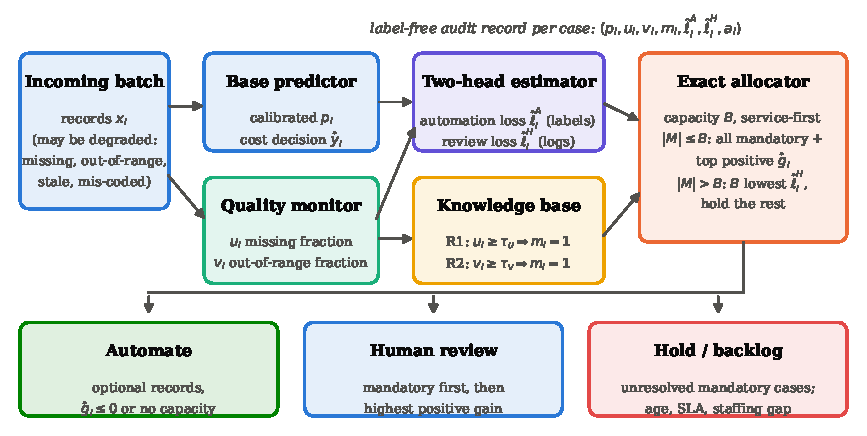
\includegraphics[width=1\textwidth,height=\textheight]{budgeted_deferral/figs/fig1_framework.pdf}
\caption{Fig. 1. Architecture of the governance-constrained routing
system. The quality monitor feeds both the rule base and the loss
estimator; the allocator enforces capacity and the service-first
constraint, and held records form a backlog.}
\end{figure}

\hypertarget{experimental-design}{%
\section{4. Experimental design}\label{experimental-design}}

\hypertarget{datasets-and-partitions}{%
\subsection{4.1. Datasets and
partitions}\label{datasets-and-partitions}}

Credit decisions are an established benchmarking domain {[}42{]}. We use
three public credit datasets from the earlier draft and one external
dataset: German numeric credit (1,000 records, 24 numeric predictors;
class 2 recoded to 1) {[}43{]}, Australian credit (690 records, 14
predictors) {[}44{]}, default of credit-card clients (30,000 records, 23
predictors; identifier removed) {[}45{]}, and HMEQ home-equity loans
(5,960 records, 12 predictors, default indicator) {[}46{]}. HMEQ was not
used during development. Unlike the other three datasets it contains
naturally occurring missing values in 11 of 12 predictors, so it tests
the method on real rather than injected incompleteness. Its two
categorical fields are integer-coded.

Feature-identical records, including those with conflicting labels, are
grouped before splitting. Groups are stratified by majority label into
about 45\% predictor training, 15\% calibration, 20\% gain fitting and
20\% testing, so no feature vector crosses roles. Twenty seeds (2--21)
define the evaluation splits. Seeds 0--1 were used during the original
development and are excluded.

\hypertarget{base-predictor-and-estimators}{%
\subsection{4.2. Base predictor and
estimators}\label{base-predictor-and-estimators}}

The base predictor is a histogram gradient-boosting classifier (at most
120 iterations, 15 leaves, learning rate 0.07, L2 penalty 1) trained on
clean predictor-training rows. It handles missing values natively.
Calibration is logistic regression on clipped log-odds, fitted on the
calibration partition expanded into clean, missing, outlier and mixed
versions. Loss heads are histogram gradient-boosting regressors (at most
100 iterations, seven leaves, learning rate 0.06, L2 penalty 5, minimum
leaf size \(\max(20,\lfloor N/200\rfloor)\)), fitted on the gain
partition expanded in the same four ways. All bounds and medians come
from predictor-training rows. Software: scikit-learn 1.9.1, NumPy 2.5
and SciPy 1.18.

\hypertarget{data-quality-conditions}{%
\subsection{4.3. Data-quality
conditions}\label{data-quality-conditions}}

Test partitions are evaluated under nine conditions (Table 2). Family A
reproduces the earlier protocol: defects that completeness and range
checks can see. Family B adds domain-valid defects that are common in
business data but largely invisible to such checks. All corruption is
applied at test time, and Family B mechanisms never appear in
calibration or gain fitting, so Family B also tests generalisation to
unseen defect mechanisms. Code-like fields are those with at most ten
distinct training values.

\begin{longtable}[]{@{}
  >{\raggedright\arraybackslash}p{(\columnwidth - 6\tabcolsep) * \real{0.2500}}
  >{\raggedright\arraybackslash}p{(\columnwidth - 6\tabcolsep) * \real{0.2500}}
  >{\raggedright\arraybackslash}p{(\columnwidth - 6\tabcolsep) * \real{0.2500}}
  >{\raggedright\arraybackslash}p{(\columnwidth - 6\tabcolsep) * \real{0.2500}}@{}}
\caption{Table 2. Data-quality conditions. Family A defects are visible
to completeness and range checks; Family B defects are domain-valid and
largely invisible to them. Family B mechanisms are never used for
fitting.}\tabularnewline
\toprule\noalign{}
\begin{minipage}[b]{\linewidth}\raggedright
Family
\end{minipage} & \begin{minipage}[b]{\linewidth}\raggedright
Condition
\end{minipage} & \begin{minipage}[b]{\linewidth}\raggedright
Mechanism (per test record)
\end{minipage} & \begin{minipage}[b]{\linewidth}\raggedright
Visible to \(u,v\)?
\end{minipage} \\
\midrule\noalign{}
\endfirsthead
\toprule\noalign{}
\begin{minipage}[b]{\linewidth}\raggedright
Family
\end{minipage} & \begin{minipage}[b]{\linewidth}\raggedright
Condition
\end{minipage} & \begin{minipage}[b]{\linewidth}\raggedright
Mechanism (per test record)
\end{minipage} & \begin{minipage}[b]{\linewidth}\raggedright
Visible to \(u,v\)?
\end{minipage} \\
\midrule\noalign{}
\endhead
\bottomrule\noalign{}
\endlastfoot
--- & clean & none (HMEQ: natural missingness) & --- \\
A & missing & each cell missing with probability \(r\sim U[0,0.55]\) &
yes \\
A & outliers & cells with probability \(r\sim U[0,0.18]\) offset by
\(\pm U[1.2,2.5]\,t_j\) & mostly \\
A & mixed & outliers \(r\sim U[0,0.12]\), then missing
\(r\sim U[0,0.35]\) & yes \\
A & shift (severe) & outliers \(r\sim U[0.08,0.25]\), then missing
\(r\sim U[0.35,0.75]\) & yes \\
B & informative missing & missing rate \(r\sim U[0,0.35]\) scaled by 1.8
if \(y=1\), 0.6 if \(y=0\) (MNAR) & partly \\
B & stale & with probability 0.5 a record's continuous fields are
deflated by a common factor \(U[0.55,0.90]\) (outdated snapshot) &
rarely \\
B & inconsistent codes & code-like cells with probability
\(r\sim U[0,0.30]\) replaced by a different valid code & no \\
B & realistic mix & stale (0.3) + inconsistent (\(U[0,0.15]\)) +
informative missing (\(U[0,0.20]\)) & partly \\
\end{longtable}

\hypertarget{reviewer-models-and-feedback}{%
\subsection{4.4. Reviewer models and
feedback}\label{reviewer-models-and-feedback}}

Because no reviewer logs are available for these public datasets,
reviewer behaviour is simulated. To avoid favouring the proposed
representation we use five models (Table 3), only one of which depends
on the router's quality signals. All are symmetric: the reviewer returns
the wrong label with probability \(e_i\).

\begin{longtable}[]{@{}
  >{\raggedright\arraybackslash}p{(\columnwidth - 4\tabcolsep) * \real{0.3333}}
  >{\raggedright\arraybackslash}p{(\columnwidth - 4\tabcolsep) * \real{0.3333}}
  >{\raggedright\arraybackslash}p{(\columnwidth - 4\tabcolsep) * \real{0.3333}}@{}}
\caption{Table 3. Simulated reviewer models. The feature-dependent and
AI-correlated reviewers err on information the router does not observe;
the AI-correlated reviewer errs most where the model
errs.}\tabularnewline
\toprule\noalign{}
\begin{minipage}[b]{\linewidth}\raggedright
Reviewer
\end{minipage} & \begin{minipage}[b]{\linewidth}\raggedright
Error probability \(e_i\)
\end{minipage} & \begin{minipage}[b]{\linewidth}\raggedright
Depends on router's \((u,v)\)?
\end{minipage} \\
\midrule\noalign{}
\endfirsthead
\toprule\noalign{}
\begin{minipage}[b]{\linewidth}\raggedright
Reviewer
\end{minipage} & \begin{minipage}[b]{\linewidth}\raggedright
Error probability \(e_i\)
\end{minipage} & \begin{minipage}[b]{\linewidth}\raggedright
Depends on router's \((u,v)\)?
\end{minipage} \\
\midrule\noalign{}
\endhead
\bottomrule\noalign{}
\endlastfoot
constant & 0.10 & no \\
quality-coupled (earlier draft) & \(\min(0.40,\,0.05+0.35u_i+0.25v_i)\)
& yes \\
feature-dependent & \(0.02+0.24\,\Phi(1.5\,\tilde z_i)\), where
\(\tilde z_i\) is a standardised hidden random projection of the
\emph{clean} features & no \\
AI-correlated &
\(\min(0.45,\,0.05+0.25\,\mathbb{1}[\hat y_i\ne y_i]+0.10(1-\lvert 2p^{clean}_i-1\rvert))\)
& no \\
adverse & 0.25 & no \\
\end{longtable}

The earlier draft trained gain models on expected reviewer losses for
every record, which is optimistic. In the main protocol here
(\textbf{logs}), a random 40\% of gain-fitting records have a review
log, and each log contains one sampled reviewer decision. Labels are
available for all gain-fitting records. Every learned method is trained
under this protocol. The optimistic protocol (\textbf{oracle targets})
is rerun for comparison, and the logged fraction is varied from 10\% to
100\% in Section 5.5.

\hypertarget{methods-compared}{%
\subsection{4.5. Methods compared}\label{methods-compared}}

All methods share the base predictor, the automated decision
\(\hat y_i\), the rule base, capacity and costs. They differ only in how
they rank records for review (Table 4). Rule-constrained heuristics fill
all remaining capacity. Learned methods review an optional record only
if their own deferral criterion is positive. Because the published L2D
methods have no notion of a hold, every method uses its own score to
order mandatory records under overload, and the overload-ordering rule
is ablated separately. In the L2D baselines only the rejector is used;
the automated decision remains the shared \(\hat y_i\), so that
differences reflect routing rather than classifier quality.

\begin{longtable}[]{@{}
  >{\raggedright\arraybackslash}p{(\columnwidth - 6\tabcolsep) * \real{0.2500}}
  >{\raggedright\arraybackslash}p{(\columnwidth - 6\tabcolsep) * \real{0.2500}}
  >{\raggedright\arraybackslash}p{(\columnwidth - 6\tabcolsep) * \real{0.2500}}
  >{\raggedright\arraybackslash}p{(\columnwidth - 6\tabcolsep) * \real{0.2500}}@{}}
\caption{Table 4. Methods. L2D surrogates are one-hidden-layer networks
(32 ReLU units, Adam, early stopping on a 20\% validation split of
logged records) implemented in NumPy, since a deep-learning framework
was not required for tabular inputs.}\tabularnewline
\toprule\noalign{}
\begin{minipage}[b]{\linewidth}\raggedright
Method
\end{minipage} & \begin{minipage}[b]{\linewidth}\raggedright
Ranking score
\end{minipage} & \begin{minipage}[b]{\linewidth}\raggedright
Information
\end{minipage} & \begin{minipage}[b]{\linewidth}\raggedright
Source / adaptation
\end{minipage} \\
\midrule\noalign{}
\endfirsthead
\toprule\noalign{}
\begin{minipage}[b]{\linewidth}\raggedright
Method
\end{minipage} & \begin{minipage}[b]{\linewidth}\raggedright
Ranking score
\end{minipage} & \begin{minipage}[b]{\linewidth}\raggedright
Information
\end{minipage} & \begin{minipage}[b]{\linewidth}\raggedright
Source / adaptation
\end{minipage} \\
\midrule\noalign{}
\endhead
\bottomrule\noalign{}
\endlastfoot
Automation only & --- (no review, rules ignored) & --- & reference \\
Random + rules & uniform random & --- & reference \\
Confidence & \(-\lvert p_i-c_{FP}/(c_{FP}+c_{FN})\rvert\) & \(p\) &
boundary uncertainty \\
Chow cost risk & \(s_i\) & \(p\) & Chow's rule {[}7{]}; constant expert
cost \\
Quality only & \(u_i+v_i\) & \(u,v\) & reference \\
Single-head gain (earlier draft) & \(\hat g_i\) from one regressor &
\(z_i\) & logged records only \\
L2D-CE & \(g_\perp-\max_y g_y\) (softmax) & scaled \(x\), \(u,v,p\) &
Mozannar \& Sontag {[}10{]}, cost-sensitive weights \(\max_j c_j-c_k\),
MLP(32) \\
L2D-OvA & \(\sigma(g_\perp)-\max_y\sigma(g_y)\) & scaled \(x\),
\(u,v,p\) & Verma \& Nalisnick {[}11{]}, examples weighted by \(w(y)\),
MLP(32) \\
Differential triage & \(\hat\ell^A-\hat\ell^H-c_R\), ordered by gain &
\(p\), \(u,v\), raw \(x\) & Raghu et al.~{[}13{]}, two error models \\
Two-head, probability only & as proposed & \(p,s\) & quality ablation \\
\textbf{Two-head, quality-aware (proposed)} & \(\hat g_i\); overload by
\(\hat\ell^H_i\) & \(z_i\) & this paper \\
Oracle & true \(g_i\), true \(\ell^H_i\) & labels & upper bound, not
deployable \\
\end{longtable}

\hypertarget{metrics-statistics-and-hypotheses}{%
\subsection{4.6. Metrics, statistics and
hypotheses}\label{metrics-statistics-and-hypotheses}}

The primary metric is expected cost per record (Eq. 4), evaluated with
true labels and expected reviewer losses. We also report review, hold
and violation rates (a violation is an automated mandatory record). The
primary comparison averages the three original datasets equally over the
eight non-clean conditions and all five reviewer models at 20\%
capacity. Reviewer-specific and family-specific results are reported
separately, and HMEQ is reported as an external check.

Repeated splits reuse observations, so ordinary paired \(t\) intervals
are too narrow. We use the corrected resampled \(t\)-test of Nadeau and
Bengio {[}47{]}, which inflates the variance of the \(J=20\) split-level
differences by \((1/J + n_{test}/n_{train})\) with
\(n_{test}/n_{train}=0.25\). Holm's procedure {[}48{]} adjusts the
family of planned comparisons. We also report the number of seeds (of
20) on which the proposed method has lower cost.

Before running the revised experiments we fixed four hypotheses:

\begin{itemize}
\tightlist
\item
  \textbf{H1 (coupled value).} Quality-aware two-head routing has lower
  cost than probability-only two-head routing when reviewer error
  depends on observable quality and defects are visible (quality-coupled
  reviewer, Family A).
\item
  \textbf{H2 (decoupled null).} The advantage shrinks toward zero when
  reviewer error does not depend on observable quality or when defects
  are invisible (Family B).
\item
  \textbf{H3 (overload ordering).} Under severe shift, ordering
  mandatory records by \(\hat\ell^H\) yields lower cost than ordering by
  \(\hat g\).
\item
  \textbf{H4 (log efficiency).} With incomplete logs, the two-head
  estimator has lower cost than the single-head estimator, and the
  difference narrows as logs become complete.
\end{itemize}

\hypertarget{multi-period-backlog-simulation}{%
\subsection{4.7. Multi-period backlog
simulation}\label{multi-period-backlog-simulation}}

To measure managerial outcomes we simulate 40 periods (``days'') of 100
arrivals each, drawn with replacement from the test partition. Data
quality is \emph{mixed} on days 1--10 and 21--40 and \emph{severe shift}
on days 11--20, a ten-day deterioration episode. Held mandatory records
are carried forward. The router is fitted once and not refitted.
Capacity per day ranges from 10\% to 70\% of arrivals. We compare three
prioritisation rules for mandatory records: first-in-first-out (FIFO),
the cost-exact rule of Proposition 1b (lowest \(\hat\ell^H\) first), and
the gain ordering of the earlier draft. Each held record incurs a
waiting cost of 0.25 per day, and records unresolved at day 40 incur
\(c_H=1.5\). Outcomes are cost per arrival, cost per completed case,
completion rate, backlog, waiting time (mean and 95th percentile), the
share of mandatory cases resolved within two days (SLA-2), reviewer
override rate (sampled reviewer decision differs from the model
decision), and capacity utilisation. Ten seeds per dataset are used,
with the quality-coupled and feature-dependent reviewers.

\hypertarget{results}{%
\section{5. Results}\label{results}}

\hypertarget{replication-of-the-earlier-draft}{%
\subsection{5.1. Replication of the earlier
draft}\label{replication-of-the-earlier-draft}}

We first reran the earlier protocol (oracle reviewer-loss targets,
single-head gain models, quality-coupled reviewer, Family A, 20\%
capacity) in the reimplemented pipeline. Absolute values differ from the
draft because the code was rebuilt from the manuscript description, but
the pattern is the same. Quality-aware single-head gain cost 0.6121
versus 0.6150 for feature-aware gain, a paired difference of 0.0028 in
its favour. The naive split interval was {[}−0.0009, 0.0066{]} and the
corrected interval {[}−0.0064, 0.0120{]} (p = 0.53). The draft reported
a difference of 0.0012 with interval {[}−0.0022, 0.0046{]}. As in the
draft, the advantage came from the default dataset (0.6341 vs 0.6417)
and reversed on Australian credit (0.5243 vs 0.5234). Confidence
(0.6106) and Chow cost risk (0.6105) were again at least as good.
Replacing oracle targets with noisy, incomplete logs raised the Family A
cost of every learned method by 0.2--0.7\% (0.6048→0.6085 for the
two-head model) and left the heuristics unchanged, because they use no
reviewer data.

\hypertarget{main-comparison-against-published-methods}{%
\subsection{5.2. Main comparison against published
methods}\label{main-comparison-against-published-methods}}

Table 5 reports the primary comparison: three datasets, eight non-clean
conditions and 20\% capacity, under each reviewer model. All
rule-constrained methods reviewed 19.8\% of records, held 6.0\% and had
no rule violations, so differences in cost reflect \emph{which} records
were reviewed. Among methods that learn from review logs, the proposed
two-head quality-aware router had the lowest macro cost (0.5355), ahead
of the earlier single-head design (0.5362), differential triage
(0.5372), probability-only two-head (0.5381), L2D-OvA (0.5421) and
L2D-CE (0.5461). The two simple cost-aware heuristics were lower still:
Chow cost risk at 0.5291 and confidence at 0.5295. The oracle bound
(0.3773) shows that most of the available improvement over these
heuristics remains unrealised by every method.

\begin{longtable}[]{@{}
  >{\raggedright\arraybackslash}p{(\columnwidth - 12\tabcolsep) * \real{0.1429}}
  >{\raggedright\arraybackslash}p{(\columnwidth - 12\tabcolsep) * \real{0.1429}}
  >{\raggedright\arraybackslash}p{(\columnwidth - 12\tabcolsep) * \real{0.1429}}
  >{\raggedright\arraybackslash}p{(\columnwidth - 12\tabcolsep) * \real{0.1429}}
  >{\raggedright\arraybackslash}p{(\columnwidth - 12\tabcolsep) * \real{0.1429}}
  >{\raggedright\arraybackslash}p{(\columnwidth - 12\tabcolsep) * \real{0.1429}}
  >{\raggedright\arraybackslash}p{(\columnwidth - 12\tabcolsep) * \real{0.1429}}@{}}
\caption{Table 5. Expected cost per record at 20\% capacity (lower is
better), averaged over German, Australian and default datasets, eight
non-clean conditions and 20 splits. Learned methods are trained on
noisy, incomplete review logs. Bold marks the lowest deployable cost in
each column. Automation only ignores the rules (12.6\% of records
violate them).}\tabularnewline
\toprule\noalign{}
\begin{minipage}[b]{\linewidth}\raggedright
Method
\end{minipage} & \begin{minipage}[b]{\linewidth}\raggedright
Constant
\end{minipage} & \begin{minipage}[b]{\linewidth}\raggedright
Quality-coupled
\end{minipage} & \begin{minipage}[b]{\linewidth}\raggedright
Feature-dep.
\end{minipage} & \begin{minipage}[b]{\linewidth}\raggedright
AI-correlated
\end{minipage} & \begin{minipage}[b]{\linewidth}\raggedright
Adverse
\end{minipage} & \begin{minipage}[b]{\linewidth}\raggedright
Macro
\end{minipage} \\
\midrule\noalign{}
\endfirsthead
\toprule\noalign{}
\begin{minipage}[b]{\linewidth}\raggedright
Method
\end{minipage} & \begin{minipage}[b]{\linewidth}\raggedright
Constant
\end{minipage} & \begin{minipage}[b]{\linewidth}\raggedright
Quality-coupled
\end{minipage} & \begin{minipage}[b]{\linewidth}\raggedright
Feature-dep.
\end{minipage} & \begin{minipage}[b]{\linewidth}\raggedright
AI-correlated
\end{minipage} & \begin{minipage}[b]{\linewidth}\raggedright
Adverse
\end{minipage} & \begin{minipage}[b]{\linewidth}\raggedright
Macro
\end{minipage} \\
\midrule\noalign{}
\endhead
\bottomrule\noalign{}
\endlastfoot
Automation only (no rules) & 0.5530 & 0.5530 & 0.5530 & 0.5530 & 0.5530
& 0.5530 \\
Random + rules & 0.5414 & 0.5638 & 0.5609 & 0.5689 & 0.6135 & 0.5697 \\
Confidence & 0.5033 & 0.5252 & 0.5191 & \textbf{0.5375} &
\textbf{0.5621} & 0.5295 \\
Chow cost risk & \textbf{0.5015} & \textbf{0.5242} & \textbf{0.5184} &
0.5377 & 0.5640 & \textbf{0.5291} \\
Quality only & 0.5390 & 0.5787 & 0.5615 & 0.5695 & 0.6217 & 0.5741 \\
Single-head gain (earlier draft) & 0.5081 & 0.5282 & 0.5256 & 0.5454 &
0.5736 & 0.5362 \\
L2D-CE {[}10{]} & 0.5206 & 0.5435 & 0.5300 & 0.5527 & 0.5837 & 0.5461 \\
L2D-OvA {[}11{]} & 0.5152 & 0.5418 & 0.5274 & 0.5483 & 0.5777 &
0.5421 \\
Differential triage {[}13{]} & 0.5109 & 0.5326 & 0.5231 & 0.5455 &
0.5740 & 0.5372 \\
Two-head, probability only & 0.5108 & 0.5345 & 0.5265 & 0.5458 & 0.5729
& 0.5381 \\
Two-head, quality-aware (proposed) & 0.5070 & 0.5293 & 0.5250 & 0.5425 &
0.5736 & 0.5355 \\
Oracle (uses labels; bound) & 0.3470 & 0.3628 & 0.3539 & 0.4145 & 0.4084
& 0.3773 \\
\end{longtable}

Table 6 gives the paired comparisons with corrected intervals. Against
L2D-CE the proposed router was 1.95\% cheaper on 19 of 20 splits
(corrected p = 0.014), but this does not survive Holm adjustment across
the eight planned comparisons (adjusted p = 0.11). No other difference
was significant after correction. Against Chow cost risk and confidence
the proposed method was about 1.2\% \emph{more} expensive and won on
only five and four splits. We therefore do not claim superiority over
simple cost-aware routing in the pooled comparison.

\begin{longtable}[]{@{}
  >{\raggedright\arraybackslash}p{(\columnwidth - 12\tabcolsep) * \real{0.1429}}
  >{\raggedright\arraybackslash}p{(\columnwidth - 12\tabcolsep) * \real{0.1429}}
  >{\raggedright\arraybackslash}p{(\columnwidth - 12\tabcolsep) * \real{0.1429}}
  >{\raggedright\arraybackslash}p{(\columnwidth - 12\tabcolsep) * \real{0.1429}}
  >{\raggedright\arraybackslash}p{(\columnwidth - 12\tabcolsep) * \real{0.1429}}
  >{\raggedright\arraybackslash}p{(\columnwidth - 12\tabcolsep) * \real{0.1429}}
  >{\raggedright\arraybackslash}p{(\columnwidth - 12\tabcolsep) * \real{0.1429}}@{}}
\caption{Table 6. Paired comparisons for the primary endpoint. Positive
differences favour the proposed method. Intervals and p-values use the
Nadeau--Bengio correction for overlapping training sets; Holm adjustment
is over the seven comparisons shown plus automation
only.}\tabularnewline
\toprule\noalign{}
\begin{minipage}[b]{\linewidth}\raggedright
Proposed vs.
\end{minipage} & \begin{minipage}[b]{\linewidth}\raggedright
Δ cost (comparator − proposed)
\end{minipage} & \begin{minipage}[b]{\linewidth}\raggedright
Corrected 95\% CI
\end{minipage} & \begin{minipage}[b]{\linewidth}\raggedright
Relative
\end{minipage} & \begin{minipage}[b]{\linewidth}\raggedright
Wins /20
\end{minipage} & \begin{minipage}[b]{\linewidth}\raggedright
p
\end{minipage} & \begin{minipage}[b]{\linewidth}\raggedright
Holm p
\end{minipage} \\
\midrule\noalign{}
\endfirsthead
\toprule\noalign{}
\begin{minipage}[b]{\linewidth}\raggedright
Proposed vs.
\end{minipage} & \begin{minipage}[b]{\linewidth}\raggedright
Δ cost (comparator − proposed)
\end{minipage} & \begin{minipage}[b]{\linewidth}\raggedright
Corrected 95\% CI
\end{minipage} & \begin{minipage}[b]{\linewidth}\raggedright
Relative
\end{minipage} & \begin{minipage}[b]{\linewidth}\raggedright
Wins /20
\end{minipage} & \begin{minipage}[b]{\linewidth}\raggedright
p
\end{minipage} & \begin{minipage}[b]{\linewidth}\raggedright
Holm p
\end{minipage} \\
\midrule\noalign{}
\endhead
\bottomrule\noalign{}
\endlastfoot
Single-head gain (earlier draft) & 0.0007 & {[}−0.0031, 0.0046{]} &
+0.13\% & 13 & 0.70 & 1.00 \\
L2D-CE & 0.0106 & {[}0.0024, 0.0189{]} & +1.95\% & 19 & 0.014 & 0.11 \\
L2D-OvA & 0.0066 & {[}−0.0018, 0.0151{]} & +1.22\% & 17 & 0.12 & 0.70 \\
Differential triage & 0.0018 & {[}−0.0064, 0.0100{]} & +0.33\% & 13 &
0.66 & 1.00 \\
Two-head, probability only & 0.0026 & {[}−0.0025, 0.0078{]} & +0.49\% &
13 & 0.30 & 0.89 \\
Chow cost risk & −0.0063 & {[}−0.0144, 0.0017{]} & −1.20\% & 5 & 0.12 &
0.70 \\
Confidence & −0.0060 & {[}−0.0140, 0.0020{]} & −1.13\% & 4 & 0.13 &
0.70 \\
\end{longtable}

Per dataset, the picture is consistent with a sample-size explanation
(Table 7). On the default dataset, whose gain-fitting partition contains
about 6,000 records, the proposed router beat every comparator on all 20
splits: Chow by 1.10\%, confidence by 1.37\%, L2D-CE by 1.29\% and
probability-only two-head by 1.45\% (all corrected p ≤ 0.003). On German
(about 200 gain-fitting records) and Australian credit (about 140), it
lost to Chow by 1.96\% and 3.20\%. Across all datasets and reviewer
models, the learned methods' disadvantage relative to Chow grows with
capacity (Fig. 2). This is expected: at higher capacity more marginal
records must be ranked, and noisy gain estimates matter more there.

\begin{longtable}[]{@{}
  >{\raggedright\arraybackslash}p{(\columnwidth - 8\tabcolsep) * \real{0.2000}}
  >{\raggedright\arraybackslash}p{(\columnwidth - 8\tabcolsep) * \real{0.2000}}
  >{\raggedright\arraybackslash}p{(\columnwidth - 8\tabcolsep) * \real{0.2000}}
  >{\raggedright\arraybackslash}p{(\columnwidth - 8\tabcolsep) * \real{0.2000}}
  >{\raggedright\arraybackslash}p{(\columnwidth - 8\tabcolsep) * \real{0.2000}}@{}}
\caption{Table 7. Relative cost reduction of the proposed router by
dataset at 20\% capacity (positive favours the proposed method), pooled
over eight non-clean conditions and five reviewers; wins out of 20
splits in parentheses. Bold: corrected p \textless{}
0.01.}\tabularnewline
\toprule\noalign{}
\begin{minipage}[b]{\linewidth}\raggedright
Dataset (gain-fitting records)
\end{minipage} & \begin{minipage}[b]{\linewidth}\raggedright
vs.~Chow cost risk
\end{minipage} & \begin{minipage}[b]{\linewidth}\raggedright
vs.~Confidence
\end{minipage} & \begin{minipage}[b]{\linewidth}\raggedright
vs.~L2D-CE
\end{minipage} & \begin{minipage}[b]{\linewidth}\raggedright
vs.~Two-head prob. only
\end{minipage} \\
\midrule\noalign{}
\endfirsthead
\toprule\noalign{}
\begin{minipage}[b]{\linewidth}\raggedright
Dataset (gain-fitting records)
\end{minipage} & \begin{minipage}[b]{\linewidth}\raggedright
vs.~Chow cost risk
\end{minipage} & \begin{minipage}[b]{\linewidth}\raggedright
vs.~Confidence
\end{minipage} & \begin{minipage}[b]{\linewidth}\raggedright
vs.~L2D-CE
\end{minipage} & \begin{minipage}[b]{\linewidth}\raggedright
vs.~Two-head prob. only
\end{minipage} \\
\midrule\noalign{}
\endhead
\bottomrule\noalign{}
\endlastfoot
German (≈200) & −1.96\% (3/20) & −0.98\% (7/20) & +1.84\% (16/20) &
−0.07\% (7/20) \\
Australian (≈140) & −3.20\% (3/20) & −4.81\% (1/20) & +2.94\% (16/20) &
+0.01\% (9/20) \\
Default (≈6,000) & \textbf{+1.10\% (20/20)} & \textbf{+1.37\% (20/20)} &
\textbf{+1.29\% (20/20)} & \textbf{+1.45\% (20/20)} \\
HMEQ, external (≈1,190) & +0.24\% (11/20) & −2.22\% (0/20) & +0.65\%
(14/20) & −0.03\% (12/20) \\
\end{longtable}

\begin{figure}
\centering
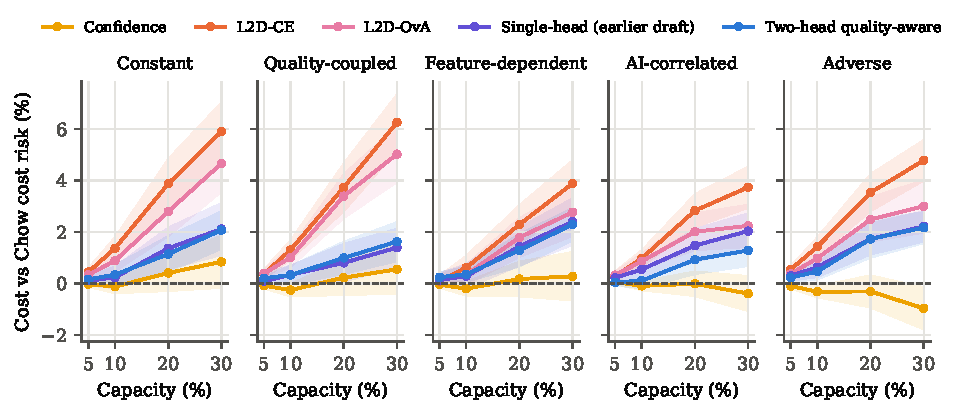
\includegraphics[width=1\textwidth,height=\textheight]{budgeted_deferral/figs/fig2_capacity.pdf}
\caption{Fig. 2. Cost of learned routers relative to Chow cost risk
across review capacity, by reviewer model (three datasets, eight
non-clean conditions, 20 splits). Bands are ±1.96 standard errors across
split means. Values above zero indicate higher cost than Chow's rule.}
\end{figure}

\hypertarget{how-much-review-data-does-a-learned-router-need}{%
\subsection{5.3. How much review data does a learned router
need?}\label{how-much-review-data-does-a-learned-router-need}}

To test the sample-size explanation directly, we subsampled the
gain-fitting partition of the default and HMEQ datasets while holding
everything else fixed (Fig. 3). With about 200 gain-fitting records, the
same size as the German partition, the proposed router was 1.96\% more
expensive than Chow on the default dataset and won on no split; L2D-CE
was 5.06\% more expensive. The gap closed at about 1,800 records
(+0.10\%, 10/20 wins) and reversed at 6,000 (−1.10\%, 20/20 wins). The
two-head quality-aware router was the best learned method at every size
on the default dataset. Its advantage over the probability-only two-head
router also grew with data (0.5 percentage points at 200 records, 1.5 at
6,000). HMEQ showed the same trend over its smaller range, from +2.47\%
at 119 records to −0.24\% at 1,192. Because each gain-fitting record
contributes four corrupted copies and 40\% of copies carry a review log,
1,800 records correspond to roughly 2,900 logged review decisions. In
this setting, then, a learned router needs a few thousand logged review
outcomes before it beats a cost-aware heuristic. Below that volume
Chow's rule is the better choice.

\begin{figure}
\centering
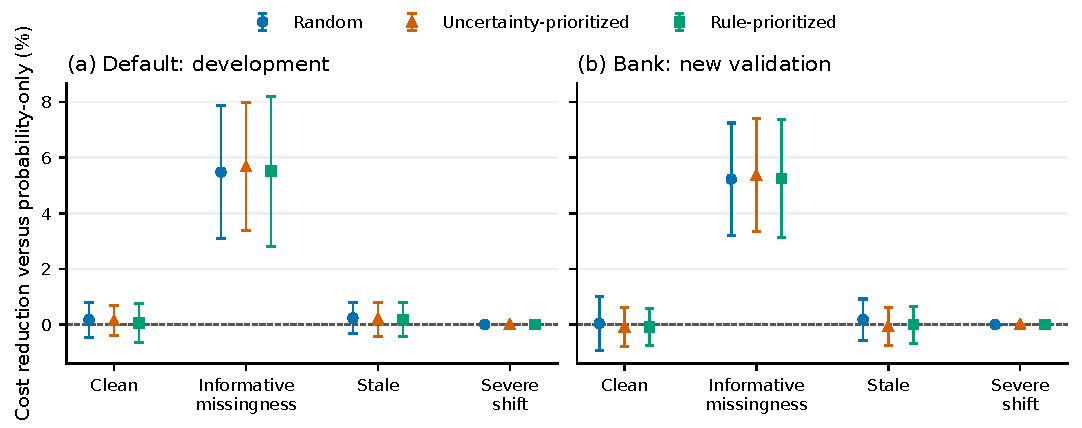
\includegraphics[width=0.96\textwidth,height=\textheight]{budgeted_deferral/figs/fig3_volume.pdf}
\caption{Fig. 3. Learned routing versus Chow's rule as the gain-fitting
partition grows (20\% capacity, eight non-clean conditions, five
reviewers, 20 splits per size). Negative values indicate lower cost than
Chow.}
\end{figure}

\hypertarget{when-does-quality-information-help}{%
\subsection{5.4. When does quality information
help?}\label{when-does-quality-information-help}}

Fig. 4 reports the cost reduction from adding quality inputs (\(u,v\)
and interactions) to the two-head router, holding everything else fixed,
for every condition × reviewer cell at 20\% capacity. The prespecified
hypotheses fare as follows.

\textbf{H1 (coupled value) was not supported at conventional
significance.} With the quality-coupled reviewer and visible defects,
quality inputs reduced cost by 0.65\% on 16 of 20 splits (corrected 95\%
CI {[}−0.0029, 0.0108{]}, p = 0.24).

\textbf{H2 (decoupled null) was supported for visible defects but not
for invisible ones.} When reviewer error did not depend on quality and
defects were visible, the effect was essentially zero: −0.07\%, 10/20
wins, p = 0.80. Contrary to H2, quality inputs helped \emph{more} under
Family B (domain-valid defects): +1.41\% with the coupled reviewer and
+0.94\% with the decoupled reviewers, neither significant. The effect
came almost entirely from one condition. Under informative missingness,
quality inputs reduced cost under every reviewer model, from +1.2\%
(adverse) to +3.5\% (constant; 17/20, p = 0.039). Pooled over reviewers
the reduction was 2.29\% (18/20, p = 0.045).

The mechanism is identified by routing quality information to only one
head (Table 8). Under informative missingness, quality inputs in the
automation-loss head alone reduced cost by 2.83\% on all 20 splits (p =
0.013), whereas quality inputs in the reviewer-loss head alone did
nothing (−0.28\%, 7/20). Missingness that depends on the outcome makes
the base predictor's error on incomplete records predictable from the
missing fraction. The quality signal therefore improves the estimate of
\emph{how wrong the automated decision is likely to be}, not of how
accurate the reviewer will be. Through the reviewer-loss head, quality
inputs helped only when reviewer error actually depended on quality:
+0.70\% (16/20, p = 0.17) with the coupled reviewer on Family A, versus
−0.41\% (7/20) with the feature-dependent reviewer. The earlier draft's
concern that its reviewer simulation favoured the quality representation
was therefore justified in direction but small in magnitude, and this
channel is not where most of the value lies.

\begin{longtable}[]{@{}
  >{\raggedright\arraybackslash}p{(\columnwidth - 6\tabcolsep) * \real{0.2500}}
  >{\raggedright\arraybackslash}p{(\columnwidth - 6\tabcolsep) * \real{0.2500}}
  >{\raggedright\arraybackslash}p{(\columnwidth - 6\tabcolsep) * \real{0.2500}}
  >{\raggedright\arraybackslash}p{(\columnwidth - 6\tabcolsep) * \real{0.2500}}@{}}
\caption{Table 8. Where quality information acts. Cost reduction
relative to the probability-only two-head router at 20\% capacity
(positive = quality inputs help); wins out of 20 splits. Bold: corrected
p \textless{} 0.05.}\tabularnewline
\toprule\noalign{}
\begin{minipage}[b]{\linewidth}\raggedright
Condition
\end{minipage} & \begin{minipage}[b]{\linewidth}\raggedright
Quality in automation head only
\end{minipage} & \begin{minipage}[b]{\linewidth}\raggedright
Quality in reviewer head only
\end{minipage} & \begin{minipage}[b]{\linewidth}\raggedright
Quality in both (proposed)
\end{minipage} \\
\midrule\noalign{}
\endfirsthead
\toprule\noalign{}
\begin{minipage}[b]{\linewidth}\raggedright
Condition
\end{minipage} & \begin{minipage}[b]{\linewidth}\raggedright
Quality in automation head only
\end{minipage} & \begin{minipage}[b]{\linewidth}\raggedright
Quality in reviewer head only
\end{minipage} & \begin{minipage}[b]{\linewidth}\raggedright
Quality in both (proposed)
\end{minipage} \\
\midrule\noalign{}
\endhead
\bottomrule\noalign{}
\endlastfoot
Informative missing (all reviewers) & \textbf{+2.83\% (20/20)} & −0.28\%
(7/20) & \textbf{+2.29\% (18/20)} \\
Stale records (all reviewers) & +0.98\% (13/20) & +0.04\% (10/20) &
+0.91\% (14/20) \\
Realistic mix (all reviewers) & +1.86\% (15/20) & −0.74\% (6/20) &
+0.91\% (14/20) \\
Family A, quality-coupled reviewer & +0.07\% (13/20) & +0.70\% (16/20) &
+0.65\% (16/20) \\
Family A, feature-dependent reviewer & +0.18\% (11/20) & −0.41\% (7/20)
& −0.34\% (4/20) \\
\end{longtable}

Stale records and inconsistent codes, which the quality monitor cannot
see (correlation between the true defect fraction and \(u+v\) of −0.01
to 0.14 for stale records and 0.14 to 0.45 for inconsistent codes),
produced small and unstable effects. They also produced almost no
mandatory reviews: at most 0.5\% of records were flagged, against
13--18\% under the missing condition.

\begin{figure}
\centering
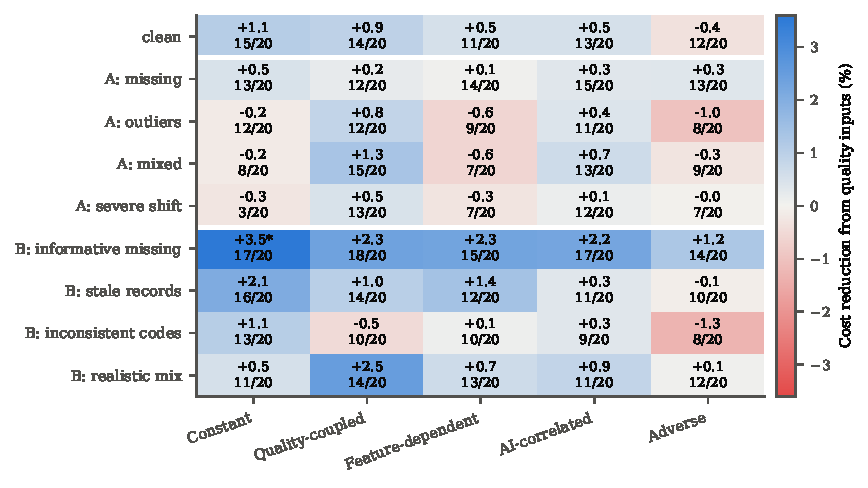
\includegraphics[width=0.82\textwidth,height=\textheight]{budgeted_deferral/figs/fig4_quality_value.pdf}
\caption{Fig. 4. Cost reduction (\%) from adding quality inputs to the
two-head router, by data condition and reviewer model, at 20\% capacity.
Each cell shows the mean over three datasets and the number of splits
(of 20) on which quality inputs helped; * marks corrected p \textless{}
0.05. Blue: quality helps; red: quality hurts.}
\end{figure}

\hypertarget{ablations-rules-overload-ordering-and-log-completeness}{%
\subsection{5.5. Ablations: rules, overload ordering and log
completeness}\label{ablations-rules-overload-ordering-and-log-completeness}}

\textbf{Rules versus quality.} Table 9 separates the quality inputs from
the rule layer. In the mixed and realistic conditions the rule layer
added 0.7--1.7\% to cost (for example 0.4614→0.4679 under mixed), the
price of reviewing flagged records instead of higher-gain optional ones.
Removing the rules left 2.1\% and 0.7\% of records automated in
violation. Under severe shift the rules forced 47.5\% of records into
holds and raised cost by 67\% (0.5987→1.0015). Without rules the router
automated 54\% of records the policy deems unfit for automation. The two
factors were roughly additive: the quality effect had the same sign with
and without rules in all three conditions.

\begin{longtable}[]{@{}
  >{\raggedright\arraybackslash}p{(\columnwidth - 12\tabcolsep) * \real{0.1429}}
  >{\raggedright\arraybackslash}p{(\columnwidth - 12\tabcolsep) * \real{0.1429}}
  >{\raggedright\arraybackslash}p{(\columnwidth - 12\tabcolsep) * \real{0.1429}}
  >{\raggedright\arraybackslash}p{(\columnwidth - 12\tabcolsep) * \real{0.1429}}
  >{\raggedright\arraybackslash}p{(\columnwidth - 12\tabcolsep) * \real{0.1429}}
  >{\raggedright\arraybackslash}p{(\columnwidth - 12\tabcolsep) * \real{0.1429}}
  >{\raggedright\arraybackslash}p{(\columnwidth - 12\tabcolsep) * \real{0.1429}}@{}}
\caption{Table 9. 2 × 2 ablation of quality inputs and the rule layer
for the two-head router (three datasets, five reviewers, 20 splits, 20\%
capacity). Unconstrained rows are diagnostic: they are cheaper because
they automate records the governance policy forbids
automating.}\tabularnewline
\toprule\noalign{}
\begin{minipage}[b]{\linewidth}\raggedright
Condition
\end{minipage} & \begin{minipage}[b]{\linewidth}\raggedright
Quality inputs
\end{minipage} & \begin{minipage}[b]{\linewidth}\raggedright
Rules
\end{minipage} & \begin{minipage}[b]{\linewidth}\raggedright
Cost
\end{minipage} & \begin{minipage}[b]{\linewidth}\raggedright
Review \%
\end{minipage} & \begin{minipage}[b]{\linewidth}\raggedright
Hold \%
\end{minipage} & \begin{minipage}[b]{\linewidth}\raggedright
Violation \%
\end{minipage} \\
\midrule\noalign{}
\endfirsthead
\toprule\noalign{}
\begin{minipage}[b]{\linewidth}\raggedright
Condition
\end{minipage} & \begin{minipage}[b]{\linewidth}\raggedright
Quality inputs
\end{minipage} & \begin{minipage}[b]{\linewidth}\raggedright
Rules
\end{minipage} & \begin{minipage}[b]{\linewidth}\raggedright
Cost
\end{minipage} & \begin{minipage}[b]{\linewidth}\raggedright
Review \%
\end{minipage} & \begin{minipage}[b]{\linewidth}\raggedright
Hold \%
\end{minipage} & \begin{minipage}[b]{\linewidth}\raggedright
Violation \%
\end{minipage} \\
\midrule\noalign{}
\endhead
\bottomrule\noalign{}
\endlastfoot
Mixed & off & on & 0.4688 & 19.8 & 0.0 & 0.0 \\
Mixed & on & on & 0.4679 & 19.8 & 0.0 & 0.0 \\
Mixed & off & off & 0.4610 & 19.8 & 0.0 & 2.2 \\
Mixed & on & off & 0.4614 & 19.8 & 0.0 & 2.1 \\
Realistic mix & off & on & 0.4782 & 19.8 & 0.0 & 0.0 \\
Realistic mix & on & on & 0.4739 & 19.8 & 0.0 & 0.0 \\
Realistic mix & off & off & 0.4748 & 19.8 & 0.0 & 0.7 \\
Realistic mix & on & off & 0.4687 & 19.8 & 0.0 & 0.7 \\
Severe shift & off & on & 1.0016 & 19.8 & 47.5 & 0.0 \\
Severe shift & on & on & 1.0015 & 19.8 & 47.5 & 0.0 \\
Severe shift & off & off & 0.6028 & 19.7 & 0.0 & 54.5 \\
Severe shift & on & off & 0.5987 & 19.6 & 0.0 & 54.2 \\
\end{longtable}

\textbf{Overload ordering (H3) was not supported empirically.} Ordering
mandatory records by \(\hat\ell^H\) (Proposition 1b) rather than by
\(\hat g\) reduced cost under severe shift by only 0.18\% (14/20, p =
0.47); with the quality-coupled reviewer the reduction was 0.47\% (p =
0.30). The correction is exact for true losses, but under severe shift
almost all mandatory records have similar estimated reviewer loss, so
the two orderings select largely the same records. Section 5.9 shows
that in a multi-period system the ordering affects waiting times far
more than cost.

\textbf{Log completeness (H4) received only directional support.} In the
primary comparison the two-head estimator was 0.13\% cheaper than the
single-head estimator (13/20, p = 0.70). In a dedicated sweep (three
datasets, mixed and realistic conditions, quality-coupled and
feature-dependent reviewers, 10 splits), the two-head estimator was
0.60\% cheaper with 10\% of records logged and 0.54\% cheaper with 40\%,
and 0.46\% more expensive with complete logs (all p \textgreater{} 0.5).
This is the direction H4 predicts, since the two-head design's advantage
is that its automation head can use unlogged records, but the effect is
too small to establish with these data.

\hypertarget{external-dataset-with-natural-missingness}{%
\subsection{5.6. External dataset with natural
missingness}\label{external-dataset-with-natural-missingness}}

On HMEQ, where 43.6\% of records have at least one naturally missing
value and DEBTINC is missing for 21.3\% of records, the quality-aware
router was evaluated without any injected corruption (Table 10,
``natural'' column). There it was cheaper than the probability-only
two-head router (0.2053 vs 0.2163; 19/20 splits, corrected p = 0.019)
and than Chow cost risk (0.2288; 19/20, p \textless{} 0.001). This
matches the informative-missingness mechanism above: natural missingness
in HMEQ is associated with default. Confidence ranking was cheaper still
(0.1847; the proposed router won on 2 of 20 splits). Under the rules,
3.3\% of HMEQ records were mandatory in the natural condition. Pooled
over all nine HMEQ conditions, confidence (0.3950) and differential
triage (0.4027) had the lowest deployable costs, and the proposed router
(0.4056) was 0.9\% below Chow (0.4091).

\begin{longtable}[]{@{}
  >{\raggedright\arraybackslash}p{(\columnwidth - 18\tabcolsep) * \real{0.1000}}
  >{\raggedright\arraybackslash}p{(\columnwidth - 18\tabcolsep) * \real{0.1000}}
  >{\raggedright\arraybackslash}p{(\columnwidth - 18\tabcolsep) * \real{0.1000}}
  >{\raggedright\arraybackslash}p{(\columnwidth - 18\tabcolsep) * \real{0.1000}}
  >{\raggedright\arraybackslash}p{(\columnwidth - 18\tabcolsep) * \real{0.1000}}
  >{\raggedright\arraybackslash}p{(\columnwidth - 18\tabcolsep) * \real{0.1000}}
  >{\raggedright\arraybackslash}p{(\columnwidth - 18\tabcolsep) * \real{0.1000}}
  >{\raggedright\arraybackslash}p{(\columnwidth - 18\tabcolsep) * \real{0.1000}}
  >{\raggedright\arraybackslash}p{(\columnwidth - 18\tabcolsep) * \real{0.1000}}
  >{\raggedright\arraybackslash}p{(\columnwidth - 18\tabcolsep) * \real{0.1000}}@{}}
\caption{Table 10. HMEQ external dataset at 20\% capacity (expected cost
per record, five reviewers, 20 splits). The outliers column is omitted
for space but included in the mean. ``Natural'' applies no injected
corruption.}\tabularnewline
\toprule\noalign{}
\begin{minipage}[b]{\linewidth}\raggedright
Method
\end{minipage} & \begin{minipage}[b]{\linewidth}\raggedright
Natural
\end{minipage} & \begin{minipage}[b]{\linewidth}\raggedright
Missing
\end{minipage} & \begin{minipage}[b]{\linewidth}\raggedright
Mixed
\end{minipage} & \begin{minipage}[b]{\linewidth}\raggedright
Shift
\end{minipage} & \begin{minipage}[b]{\linewidth}\raggedright
Informative
\end{minipage} & \begin{minipage}[b]{\linewidth}\raggedright
Stale
\end{minipage} & \begin{minipage}[b]{\linewidth}\raggedright
Inconsistent
\end{minipage} & \begin{minipage}[b]{\linewidth}\raggedright
Realistic
\end{minipage} & \begin{minipage}[b]{\linewidth}\raggedright
Mean (9)
\end{minipage} \\
\midrule\noalign{}
\endfirsthead
\toprule\noalign{}
\begin{minipage}[b]{\linewidth}\raggedright
Method
\end{minipage} & \begin{minipage}[b]{\linewidth}\raggedright
Natural
\end{minipage} & \begin{minipage}[b]{\linewidth}\raggedright
Missing
\end{minipage} & \begin{minipage}[b]{\linewidth}\raggedright
Mixed
\end{minipage} & \begin{minipage}[b]{\linewidth}\raggedright
Shift
\end{minipage} & \begin{minipage}[b]{\linewidth}\raggedright
Informative
\end{minipage} & \begin{minipage}[b]{\linewidth}\raggedright
Stale
\end{minipage} & \begin{minipage}[b]{\linewidth}\raggedright
Inconsistent
\end{minipage} & \begin{minipage}[b]{\linewidth}\raggedright
Realistic
\end{minipage} & \begin{minipage}[b]{\linewidth}\raggedright
Mean (9)
\end{minipage} \\
\midrule\noalign{}
\endhead
\bottomrule\noalign{}
\endlastfoot
Confidence & \textbf{0.1847} & 0.5148 & 0.4135 & 1.0844 & 0.3319 &
\textbf{0.2223} & \textbf{0.2038} & 0.2957 & \textbf{0.3950} \\
Chow cost risk & 0.2288 & 0.5247 & 0.4137 & 1.0871 & 0.3333 & 0.2506 &
0.2363 & 0.3029 & 0.4091 \\
Single-head gain (earlier draft) & 0.2065 & 0.5228 & 0.4192 & 1.0905 &
0.3444 & 0.2389 & 0.2226 & 0.3153 & 0.4074 \\
L2D-CE & 0.2182 & 0.5212 & 0.4215 & 1.0911 & 0.3343 & 0.2406 & 0.2336 &
0.3065 & 0.4095 \\
L2D-OvA & 0.2118 & 0.5171 & 0.4210 & 1.0890 & 0.3338 & 0.2367 & 0.2320 &
0.3048 & 0.4071 \\
Differential triage & 0.2082 & 0.5199 & \textbf{0.4107} & 1.0837 &
0.3326 & 0.2434 & 0.2227 & 0.3011 & 0.4027 \\
Two-head, probability only & 0.2163 & 0.5178 & 0.4188 & \textbf{1.0826}
& 0.3407 & 0.2447 & 0.2287 & 0.3049 & 0.4067 \\
Two-head, quality-aware & 0.2053 & 0.5187 & 0.4176 & 1.0868 & 0.3450 &
0.2370 & 0.2208 & 0.3153 & 0.4056 \\
\end{longtable}

\hypertarget{governance-rule-alternatives}{%
\subsection{5.7. Governance-rule
alternatives}\label{governance-rule-alternatives}}

Table 11 compares four rule sets for the proposed router, with the
router unchanged. Because the rules are evaluated against their own
thresholds, each rule set has zero violations by construction. To judge
whether a rule set is \emph{appropriate}, we report the share of truly
defective records (more than 20\% of cells corrupted) that were
nevertheless automated. Under severe shift, the main rules reduced
automated defective records from 80.3\% (no rules) to 32.2\% at a cost
increase of 71\%, and strict rules reduced them to 4.5\% at a cost
increase of 111\%, with 75.6\% of records held. Under the realistic mix,
whose defects are mostly invisible, even strict rules left 74.7\% of
defective records automated, because rules built on completeness and
range checks cannot see stale or mis-keyed values. Lenient rules were
nearly indistinguishable from no rules except under shift. Rule sets
shifted all ranking methods by similar amounts. Confidence had the
lowest cost under the none, lenient and main rule sets, with Chow
second. Under strict rules, where three-quarters of records are
mandatory, confidence, L2D-OvA, the proposed router and its rich-input
variant were within 0.001 of each other and all slightly below Chow.

\begin{longtable}[]{@{}
  >{\raggedright\arraybackslash}p{(\columnwidth - 10\tabcolsep) * \real{0.1667}}
  >{\raggedright\arraybackslash}p{(\columnwidth - 10\tabcolsep) * \real{0.1667}}
  >{\raggedright\arraybackslash}p{(\columnwidth - 10\tabcolsep) * \real{0.1667}}
  >{\raggedright\arraybackslash}p{(\columnwidth - 10\tabcolsep) * \real{0.1667}}
  >{\raggedright\arraybackslash}p{(\columnwidth - 10\tabcolsep) * \real{0.1667}}
  >{\raggedright\arraybackslash}p{(\columnwidth - 10\tabcolsep) * \real{0.1667}}@{}}
\caption{Table 11. Governance-rule alternatives for the proposed router
(German, Australian and default; quality-coupled and feature-dependent
reviewers; 10 splits; 20\% capacity). ``Defective records automated'' is
the share of records with more than 20\% corrupted cells that the policy
automated. The lenient row for the realistic mix equals ``none'' and is
omitted.}\tabularnewline
\toprule\noalign{}
\begin{minipage}[b]{\linewidth}\raggedright
Condition
\end{minipage} & \begin{minipage}[b]{\linewidth}\raggedright
Rule set (\(\tau_u,\tau_v\))
\end{minipage} & \begin{minipage}[b]{\linewidth}\raggedright
Mandatory \%
\end{minipage} & \begin{minipage}[b]{\linewidth}\raggedright
Cost
\end{minipage} & \begin{minipage}[b]{\linewidth}\raggedright
Hold \%
\end{minipage} & \begin{minipage}[b]{\linewidth}\raggedright
Defective records automated \%
\end{minipage} \\
\midrule\noalign{}
\endfirsthead
\toprule\noalign{}
\begin{minipage}[b]{\linewidth}\raggedright
Condition
\end{minipage} & \begin{minipage}[b]{\linewidth}\raggedright
Rule set (\(\tau_u,\tau_v\))
\end{minipage} & \begin{minipage}[b]{\linewidth}\raggedright
Mandatory \%
\end{minipage} & \begin{minipage}[b]{\linewidth}\raggedright
Cost
\end{minipage} & \begin{minipage}[b]{\linewidth}\raggedright
Hold \%
\end{minipage} & \begin{minipage}[b]{\linewidth}\raggedright
Defective records automated \%
\end{minipage} \\
\midrule\noalign{}
\endhead
\bottomrule\noalign{}
\endlastfoot
Mixed & none & 0.0 & 0.4415 & 0.0 & 80.9 \\
Mixed & lenient (0.7, 0.4) & 0.1 & 0.4424 & 0.0 & 80.9 \\
Mixed & main (0.5, 0.25) & 2.8 & 0.4533 & 0.0 & 79.3 \\
Mixed & strict (0.3, 0.15) & 23.4 & 0.5268 & 3.9 & 60.0 \\
Severe shift & none & 0.0 & 0.5888 & 0.0 & 80.3 \\
Severe shift & lenient & 19.1 & 0.6437 & 1.7 & 78.5 \\
Severe shift & main & 67.8 & 1.0093 & 48.0 & 32.2 \\
Severe shift & strict & 95.5 & 1.2413 & 75.6 & 4.5 \\
Realistic mix & none & 0.0 & 0.4395 & 0.0 & 80.8 \\
Realistic mix & main & 0.8 & 0.4449 & 0.0 & 80.3 \\
Realistic mix & strict & 6.4 & 0.4763 & 0.0 & 74.7 \\
\end{longtable}

\hypertarget{cost-settings-with-re-optimisation}{%
\subsection{5.8. Cost settings with
re-optimisation}\label{cost-settings-with-re-optimisation}}

In contrast to the earlier draft's fixed-route sensitivity, here every
cost change refits the decision threshold, the loss heads and the L2D
surrogates (Table 12). The ranking was stable. Confidence had the lowest
cost in all seven settings, Chow was second, and the proposed router was
third, 0.4--1.2\% above Chow. It remained ahead of the probability-only
router, the single-head router and both L2D surrogates in every setting.
Changing the hold penalty from 0.5 to 3.0 raised the proposed router's
cost by 0.3998, equal to 2.5 × its 16.0\% hold rate, with identical
review and hold rates. This confirms empirically the invariance in
Proposition 1: under the service-first constraint, the hold penalty
changes the price of overload but not the routes.

\begin{longtable}[]{@{}
  >{\raggedright\arraybackslash}p{(\columnwidth - 14\tabcolsep) * \real{0.1250}}
  >{\raggedright\arraybackslash}p{(\columnwidth - 14\tabcolsep) * \real{0.1250}}
  >{\raggedright\arraybackslash}p{(\columnwidth - 14\tabcolsep) * \real{0.1250}}
  >{\raggedright\arraybackslash}p{(\columnwidth - 14\tabcolsep) * \real{0.1250}}
  >{\raggedright\arraybackslash}p{(\columnwidth - 14\tabcolsep) * \real{0.1250}}
  >{\raggedright\arraybackslash}p{(\columnwidth - 14\tabcolsep) * \real{0.1250}}
  >{\raggedright\arraybackslash}p{(\columnwidth - 14\tabcolsep) * \real{0.1250}}
  >{\raggedright\arraybackslash}p{(\columnwidth - 14\tabcolsep) * \real{0.1250}}@{}}
\caption{Table 12. Expected cost after re-optimising all methods for
each cost setting (German, Australian and default; mixed, shift and
realistic conditions; two reviewers; 10 splits; 20\% capacity). Small
datasets dominate this average; see Table 7 for the dataset-size
dependence.}\tabularnewline
\toprule\noalign{}
\begin{minipage}[b]{\linewidth}\raggedright
Setting
\end{minipage} & \begin{minipage}[b]{\linewidth}\raggedright
Chow
\end{minipage} & \begin{minipage}[b]{\linewidth}\raggedright
Confidence
\end{minipage} & \begin{minipage}[b]{\linewidth}\raggedright
Proposed
\end{minipage} & \begin{minipage}[b]{\linewidth}\raggedright
Two-head prob.
\end{minipage} & \begin{minipage}[b]{\linewidth}\raggedright
Single-head
\end{minipage} & \begin{minipage}[b]{\linewidth}\raggedright
L2D-CE
\end{minipage} & \begin{minipage}[b]{\linewidth}\raggedright
L2D-OvA
\end{minipage} \\
\midrule\noalign{}
\endfirsthead
\toprule\noalign{}
\begin{minipage}[b]{\linewidth}\raggedright
Setting
\end{minipage} & \begin{minipage}[b]{\linewidth}\raggedright
Chow
\end{minipage} & \begin{minipage}[b]{\linewidth}\raggedright
Confidence
\end{minipage} & \begin{minipage}[b]{\linewidth}\raggedright
Proposed
\end{minipage} & \begin{minipage}[b]{\linewidth}\raggedright
Two-head prob.
\end{minipage} & \begin{minipage}[b]{\linewidth}\raggedright
Single-head
\end{minipage} & \begin{minipage}[b]{\linewidth}\raggedright
L2D-CE
\end{minipage} & \begin{minipage}[b]{\linewidth}\raggedright
L2D-OvA
\end{minipage} \\
\midrule\noalign{}
\endhead
\bottomrule\noalign{}
\endlastfoot
FN:FP = 2:1 & 0.4877 & \textbf{0.4874} & 0.4925 & 0.4946 & 0.4945 &
0.5025 & 0.5008 \\
FN:FP = 5:1 (main) & 0.6320 & \textbf{0.6314} & 0.6358 & 0.6406 & 0.6384
& 0.6476 & 0.6444 \\
FN:FP = 10:1 & 0.7216 & \textbf{0.7157} & 0.7302 & 0.7323 & 0.7339 &
0.7446 & 0.7359 \\
Review fee 0 & 0.6221 & \textbf{0.6215} & 0.6259 & 0.6307 & 0.6285 &
0.6380 & 0.6345 \\
Review fee 0.20 & 0.6618 & \textbf{0.6612} & 0.6655 & 0.6703 & 0.6681 &
0.6788 & 0.6741 \\
Hold penalty 0.5 & 0.4721 & \textbf{0.4715} & 0.4759 & 0.4806 & 0.4785 &
0.4877 & 0.4844 \\
Hold penalty 3.0 & 0.8720 & \textbf{0.8714} & 0.8757 & 0.8805 & 0.8783 &
0.8875 & 0.8843 \\
\end{longtable}

\hypertarget{managerial-outcomes-in-a-multi-period-system}{%
\subsection{5.9. Managerial outcomes in a multi-period
system}\label{managerial-outcomes-in-a-multi-period-system}}

Table 13 and Fig. 5 report the 40-day simulation (four datasets, two
reviewers, ten seeds). Mandatory demand averaged 5.5\% of arrivals in
mixed periods and 70.0\% during the ten-day severe-shift episode. As
Proposition 2 predicts, the three prioritisation rules produced
identical backlogs, completion rates and capacity utilisation at every
staffing level, and cost per arrival differed by at most 0.005. The
fluid approximation predicted the peak backlog closely: 500, 300 and 200
records at 20\%, 40\% and 50\% capacity, against simulated means of
499.8, 299.7 and 199.7 (Fig. 5a). At 20\% capacity, 5.2\% of all
arrivals were still unresolved at day 40, and cost per arrival was 1.16
against 0.39 at 70\% capacity. Capacity, not routing, dominated cost
during the deterioration episode.

Prioritisation changed \emph{who} waited. FIFO ordering cut the
95th-percentile wait at 40\% capacity from 13.8 days (cost-exact
ordering) to 7.1 days and the maximum wait from 18.4 to 8.0 days. But it
reduced the share of mandatory cases resolved within two days from
65.3\% to 41.1\%, because FIFO serves old cases first and newly flagged
cases wait. The cost-exact and gain orderings behaved almost
identically, again because estimated reviewer losses vary little among
mandatory records. Reviewers overturned the automated decision in
44--49\% of reviewed cases. With a 5:1 cost ratio, the automated
decision deliberately labels many uncertain records as positive, so a
high override rate is expected and is not by itself evidence of a poor
model.

\begin{longtable}[]{@{}
  >{\raggedright\arraybackslash}p{(\columnwidth - 18\tabcolsep) * \real{0.1000}}
  >{\raggedright\arraybackslash}p{(\columnwidth - 18\tabcolsep) * \real{0.1000}}
  >{\raggedright\arraybackslash}p{(\columnwidth - 18\tabcolsep) * \real{0.1000}}
  >{\raggedright\arraybackslash}p{(\columnwidth - 18\tabcolsep) * \real{0.1000}}
  >{\raggedright\arraybackslash}p{(\columnwidth - 18\tabcolsep) * \real{0.1000}}
  >{\raggedright\arraybackslash}p{(\columnwidth - 18\tabcolsep) * \real{0.1000}}
  >{\raggedright\arraybackslash}p{(\columnwidth - 18\tabcolsep) * \real{0.1000}}
  >{\raggedright\arraybackslash}p{(\columnwidth - 18\tabcolsep) * \real{0.1000}}
  >{\raggedright\arraybackslash}p{(\columnwidth - 18\tabcolsep) * \real{0.1000}}
  >{\raggedright\arraybackslash}p{(\columnwidth - 18\tabcolsep) * \real{0.1000}}@{}}
\caption{Table 13. Multi-period managerial outcomes (40 days, 100
arrivals per day, severe-shift episode on days 11--20; four datasets,
two reviewers, ten seeds). The gain ordering of the earlier draft is
omitted; it differs from the cost-exact rule by at most 0.5 days in any
waiting-time measure and at most 0.04 in any rate.}\tabularnewline
\toprule\noalign{}
\begin{minipage}[b]{\linewidth}\raggedright
Capacity
\end{minipage} & \begin{minipage}[b]{\linewidth}\raggedright
Order
\end{minipage} & \begin{minipage}[b]{\linewidth}\raggedright
Cost / arrival
\end{minipage} & \begin{minipage}[b]{\linewidth}\raggedright
Cost / completed
\end{minipage} & \begin{minipage}[b]{\linewidth}\raggedright
Completed \%
\end{minipage} & \begin{minipage}[b]{\linewidth}\raggedright
Peak backlog
\end{minipage} & \begin{minipage}[b]{\linewidth}\raggedright
Mean wait (d)
\end{minipage} & \begin{minipage}[b]{\linewidth}\raggedright
P95 wait (d)
\end{minipage} & \begin{minipage}[b]{\linewidth}\raggedright
SLA-2 \%
\end{minipage} & \begin{minipage}[b]{\linewidth}\raggedright
Override \%
\end{minipage} \\
\midrule\noalign{}
\endfirsthead
\toprule\noalign{}
\begin{minipage}[b]{\linewidth}\raggedright
Capacity
\end{minipage} & \begin{minipage}[b]{\linewidth}\raggedright
Order
\end{minipage} & \begin{minipage}[b]{\linewidth}\raggedright
Cost / arrival
\end{minipage} & \begin{minipage}[b]{\linewidth}\raggedright
Cost / completed
\end{minipage} & \begin{minipage}[b]{\linewidth}\raggedright
Completed \%
\end{minipage} & \begin{minipage}[b]{\linewidth}\raggedright
Peak backlog
\end{minipage} & \begin{minipage}[b]{\linewidth}\raggedright
Mean wait (d)
\end{minipage} & \begin{minipage}[b]{\linewidth}\raggedright
P95 wait (d)
\end{minipage} & \begin{minipage}[b]{\linewidth}\raggedright
SLA-2 \%
\end{minipage} & \begin{minipage}[b]{\linewidth}\raggedright
Override \%
\end{minipage} \\
\midrule\noalign{}
\endhead
\bottomrule\noalign{}
\endlastfoot
20\% & FIFO & 1.161 & 1.148 & 94.8 & 499.8 & 9.8 & 20.2 & 18.5 & 48.3 \\
20\% & Cost-exact & 1.157 & 1.144 & 94.8 & 499.8 & 7.5 & 23.0 & 48.4 &
46.8 \\
40\% & FIFO & 0.634 & 0.634 & 100.0 & 299.7 & 3.4 & 7.1 & 41.1 & 48.2 \\
40\% & Cost-exact & 0.634 & 0.634 & 100.0 & 299.7 & 3.4 & 13.8 & 65.3 &
48.2 \\
50\% & FIFO & 0.516 & 0.516 & 100.0 & 199.7 & 1.7 & 3.9 & 71.8 & 47.3 \\
50\% & Cost-exact & 0.516 & 0.516 & 100.0 & 199.7 & 1.7 & 10.0 & 78.4 &
47.3 \\
70\% & FIFO & 0.389 & 0.389 & 100.0 & 26.8 & 0.1 & 0.5 & 100.0 & 45.6 \\
70\% & Cost-exact & 0.389 & 0.389 & 100.0 & 26.8 & 0.1 & 0.9 & 98.2 &
45.6 \\
\end{longtable}

\begin{figure}
\centering
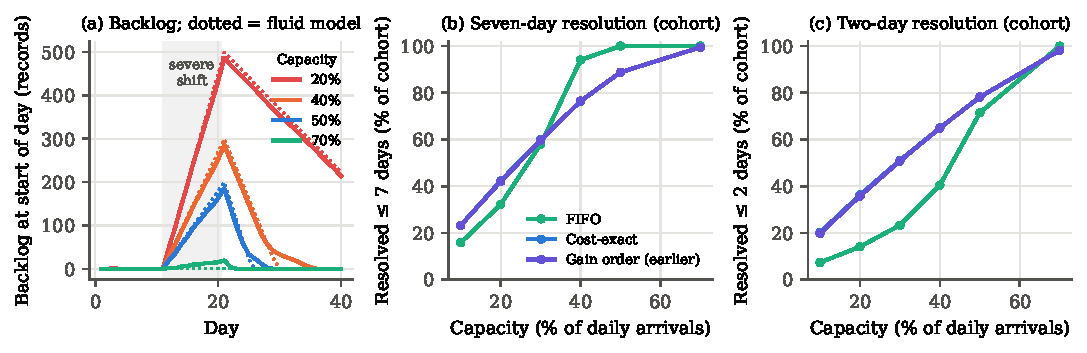
\includegraphics[width=1\textwidth,height=\textheight]{budgeted_deferral/figs/fig5_backlog.pdf}
\caption{Fig. 5. Multi-period simulation. (a) Backlog over time (seed 2,
quality-coupled reviewer, mean of four datasets) at four staffing
levels, with the fluid approximation dotted; the shaded band is the
severe-shift episode. (b) 95th-percentile waiting time and (c) share of
mandatory cases resolved within two days, by prioritisation rule,
averaged over four datasets, two reviewers and ten seeds.}
\end{figure}

\hypertarget{discussion}{%
\section{6. Discussion}\label{discussion}}

\hypertarget{answer-to-the-research-question}{%
\subsection{6.1. Answer to the research
question}\label{answer-to-the-research-question}}

The research question asked under what data-quality and review-capacity
conditions quality-aware deferral improves decision cost and service
completion while satisfying explicit governance rules. The evidence
supports a conditional answer with four parts.

First, \textbf{quality information pays when missingness is informative
about the outcome.} In that case it improves the estimate of
automated-decision error, not of reviewer error. This was the only
condition with a consistent effect across all five reviewer models
(+1.2\% to +3.5\%), and it reappeared on the external HMEQ data, where
missingness is natural rather than injected. When defects were visible
but uninformative about the outcome, or invisible to completeness and
range checks, quality inputs added little and sometimes hurt.

Second, \textbf{learned routing pays only with enough review history.}
Holding information, rules and costs fixed, every learned router,
including the published L2D surrogates, was worse than Chow's cost-risk
rule when trained on a few hundred records. The proposed router overtook
Chow at roughly 1,800 gain-fitting records (about 2,900 logged review
decisions) and beat every comparator on all splits at 6,000. The pooled
comparison in Table 5, in which two of three datasets are small,
therefore understates what a learned router achieves at operational data
volumes and overstates it for small portfolios.

Third, \textbf{capacity, not ranking, decides service completion under
deterioration.} When mandatory demand exceeded capacity, the backlog was
fully determined by staffing (Proposition 2), and the fluid rule
\((\mu-b)^+n\) predicted the peak backlog to within 0.3 records. Ranking
methods moved cost by about 1\%; moving capacity from 20\% to 40\%
during the episode cut cost per arrival by 45\% and eliminated
unresolved cases.

Fourth, \textbf{governance rules built on observable quality checks
protect against visible defects only.} They prevented the automation of
most severely degraded records under visible shift, at a substantial
service cost, but let three-quarters of records with invisible defects
through even under strict thresholds.

\hypertarget{implications-for-knowledge-based-decision-systems}{%
\subsection{6.2. Implications for knowledge-based decision
systems}\label{implications-for-knowledge-based-decision-systems}}

The study separates three components that are often conflated in
deferral systems: a \emph{knowledge layer} that encodes non-negotiable
policy, an \emph{estimation layer} that predicts the value of review,
and an \emph{allocation layer} that enforces capacity. Proposition 1
shows that once the policy is fixed and estimates are given, allocation
is a sorting problem with an exact solution in both regimes. The design
effort should therefore go into estimation and into the rules
themselves, not into the allocator. The mechanism analysis (Table 8)
adds a design principle: quality signals belong in the model of
\emph{automated} error when missingness may be informative, and in the
model of \emph{reviewer} error only when there is evidence that
reviewers are affected by the same defects. The two-head decomposition
makes that choice explicit and auditable, and lets the automation head
use all labelled outcomes even when review logs are sparse.

The results also qualify the value of methodological sophistication in
this setting. Two consistent L2D surrogates, adapted only by adding cost
weights and a shared classifier, were the weakest learned methods at
small and medium data volumes. This is unsurprising given that they
learn a three-way decision from scratch, whereas the two-head router and
Chow's rule start from a calibrated probability, but it suggests that
reviews of deferral methods should report sample-size dependence
alongside asymptotic guarantees.

\hypertarget{implications-for-managers}{%
\subsection{6.3. Implications for
managers}\label{implications-for-managers}}

Four operational recommendations follow, each tied to a measured
outcome:

\begin{enumerate}
\def\labelenumi{\arabic{enumi}.}
\tightlist
\item
  \textbf{Start with a cost-aware heuristic.} Until a few thousand
  review outcomes have been logged, route by Bayes risk of the automated
  decision (Chow's rule) or by closeness to the cost threshold. Both use
  no reviewer data, cannot overfit review logs, and were within about
  1\% of the best learned router in most settings.
\item
  \textbf{Staff to mandatory demand, not to average demand.} Review
  capacity must exceed the mandatory arrival rate during deterioration
  episodes, or a backlog of \((\mu-b)^+\) per record per period
  accumulates. In our simulation a ten-day episode at 70\% mandatory
  demand left about 500 records waiting at 20\% capacity and about 27 at
  70\%. Monitoring the mandatory rate is a leading indicator of staffing
  gaps.
\item
  \textbf{Choose the queue discipline for its service profile, not its
  cost.} FIFO halves tail waiting time; cost-ordered queues resolve more
  cases within two days but let some cases wait more than two weeks. The
  choice belongs in the service-level agreement.
\item
  \textbf{Do not treat override rates or zero violations as evidence of
  good governance.} With asymmetric costs, reviewers overturned nearly
  half of automated decisions by design. Zero rule violations held by
  construction even when three-quarters of defective records were
  automated under invisible defects. Governance reporting should include
  defect-detection coverage, unresolved-case age and the
  mandatory-to-capacity ratio.
\end{enumerate}

\hypertarget{limitations-and-future-work}{%
\section{7. Limitations and future
work}\label{limitations-and-future-work}}

\textbf{Simulated reviewers.} No public dataset links credit decisions
to logged human reviews, so reviewer behaviour is simulated. We reduced
dependence on any single assumption by using five reviewer models, two
of which err on information the router cannot see, and by training on
sampled rather than expected reviewer outcomes. Real reviewers may also
learn, tire, anchor on the model's recommendation {[}30{]} or change
behaviour under backlog pressure, none of which is modelled. Validation
with operational review logs is the most important next step.

\textbf{Datasets and corruption.} The three original benchmarks are old
and small, and Family B mechanisms are stylised versions of real
defects. HMEQ provides natural missingness but is itself a public
benchmark of uncertain provenance. Category codes are treated as
integers, and no contemporary dataset could be obtained in the computing
environment used for this revision. Results for invisible defects depend
on how stale and mis-keyed values are generated.

\textbf{Rules and costs.} Thresholds, the 5:1 cost ratio, the review fee
and the hold penalty are illustrative rather than elicited from an
organisation. We varied each and refitted the policies, and the method
ranking was stable, but appropriate values must come from domain owners
and regulators. The defect-based appropriateness measure in Table 11
uses an arbitrary 20\% threshold.

\textbf{Statistics.} Repeated splits reuse observations. The corrected
resampled \(t\)-test reduces but does not eliminate the resulting
optimism, and with three primary datasets, dataset-level generalisation
rests largely on the data-volume and external analyses. Several effects
of interest (H1, H3, H4) were directionally consistent but not
significant, and should be treated as inconclusive rather than as
evidence of no effect.

\textbf{Scope of the method.} The allocator is exact for the stated
single-batch problem, but the multi-period system uses it myopically,
without anticipating future arrivals. Congestion-aware deferral {[}28{]}
and constraint-programming assignment {[}15{]} address related dynamic
and multi-expert problems. The L2D baselines were adapted (shared
classifier, cost weights, a small network) and may perform better with
tuning or larger architectures. Fairness, legal sufficiency of the rules
and causal effects of review on outcomes are outside the scope of this
study.

\hypertarget{conclusion}{%
\section{8. Conclusion}\label{conclusion}}

This study re-examined a data-quality-aware deferral system with
explicit governance rules and review capacity, against published
deferral methods, under reviewer models that do not favour its
representation and under defects that quality checks cannot see. The
system's allocator solves the governance-constrained routing problem
exactly in both feasible and overloaded regimes, and its two-head
estimator learns from incomplete review logs. It did not, however,
outperform simple cost-aware routing in the pooled comparison dominated
by small datasets. Its value is conditional. It outperformed all
comparators when trained on several thousand records, and quality
information improved it chiefly when missingness was informative about
outcomes, through better estimates of automated error rather than of
reviewer error. Under severe data deterioration, staffing determined
backlog and service completion far more than any routing choice, and
quality-triggered rules protected only against the defects they could
observe. For knowledge-based decision systems used in AI governance, the
practical message is to make the rule layer, the estimation layer and
the capacity layer separately visible, to measure each, and to reserve
learned routing for settings with sufficient review history.

\hypertarget{data-and-code-availability}{%
\section{Data and code availability}\label{data-and-code-availability}}

All data are public: German, Australian and default credit from the UCI
Machine Learning Repository {[}43--45{]} and HMEQ {[}46{]}. The code,
configuration, seed-level results for every experiment, and scripts that
regenerate every table and figure are in the
\texttt{budgeted\_deferral/} directory of the author's repository
https://github.com/ykunam/data-quality-budgeted-deferral. A versioned
release with an archival DOI should be created before submission.

\hypertarget{declaration-of-competing-interest}{%
\section{Declaration of competing
interest}\label{declaration-of-competing-interest}}

The author must confirm before submission. No funding or competing
interests are asserted in this draft.

\hypertarget{funding}{%
\section{Funding}\label{funding}}

To be confirmed by the author before submission.

\hypertarget{credit-authorship-contribution-statement}{%
\section{CRediT authorship contribution
statement}\label{credit-authorship-contribution-statement}}

\textbf{Yeshwanth Reddy Kunam:} Conceptualization, Methodology,
Software, Validation, Formal analysis, Investigation, Data curation,
Writing -- original draft, Writing -- review and editing, Visualization.
(To be confirmed by the author.)

\hypertarget{declaration-of-generative-ai-and-ai-assisted-technologies-in-the-manuscript-preparation-process}{%
\section{Declaration of generative AI and AI-assisted technologies in
the manuscript preparation
process}\label{declaration-of-generative-ai-and-ai-assisted-technologies-in-the-manuscript-preparation-process}}

ChatGPT (OpenAI) assisted with the original study design, code and
drafting. Claude (Anthropic) assisted with the revision: reimplementing
the experimental pipeline, implementing the comparison methods, running
the experiments, statistical analysis, figures, literature checking and
manuscript drafting. The author must critically review, verify and adopt
all content before submission and takes full responsibility for the
accuracy and originality of the published work.

\hypertarget{references}{%
\section*{References}\label{references}}
\addcontentsline{toc}{section}{References}

{[}1{]} R. Abraham, J. Schneider, J. vom Brocke, Data governance: A
conceptual framework, structured review, and research agenda, Int. J.
Inf. Manag. 49 (2019) 424--438.
https://doi.org/10.1016/j.ijinfomgt.2019.07.008

{[}2{]} M. Janssen, P. Brous, E. Estevez, L.S. Barbosa, T. Janowski,
Data governance: Organizing data for trustworthy artificial
intelligence, Gov.~Inf. Q. 37 (2020) 101493.
https://doi.org/10.1016/j.giq.2020.101493

{[}3{]} E. Papagiannidis, P. Mikalef, K. Conboy, Responsible artificial
intelligence governance: A review and research framework, J. Strateg.
Inf. Syst. 34 (2025) 101885. https://doi.org/10.1016/j.jsis.2024.101885

{[}4{]} B.W. Wirtz, J.C. Weyerer, I. Kehl, Governance of artificial
intelligence: A risk and guideline-based integrative framework,
Gov.~Inf. Q. 39 (2022) 101685. https://doi.org/10.1016/j.giq.2022.101685

{[}5{]} European Parliament and Council, Regulation (EU) 2024/1689
laying down harmonised rules on artificial intelligence (Artificial
Intelligence Act), Off. J. Eur. Union L, 2024/1689, 12 July 2024, Art.
14 and Annex III(5)(b).

{[}6{]} B. Green, The flaws of policies requiring human oversight of
government algorithms, Comput. Law Secur. Rev.~45 (2022) 105681.
https://doi.org/10.1016/j.clsr.2022.105681

{[}7{]} C. Chow, On optimum recognition error and reject tradeoff, IEEE
Trans. Inf. Theory 16 (1970) 41--46.
https://doi.org/10.1109/TIT.1970.1054406

{[}8{]} X.Y. Zhang, G.S. Xie, X. Li, T. Mei, C.L. Liu, A survey on
learning to reject, Proc. IEEE 111 (2023) 185--215.
https://doi.org/10.1109/JPROC.2023.3238024

{[}9{]} D. Madras, T. Pitassi, R. Zemel, Predict responsibly: Improving
fairness and accuracy by learning to defer, in: Adv. Neural Inf.
Process. Syst. 31 (2018).

{[}10{]} H. Mozannar, D. Sontag, Consistent estimators for learning to
defer to an expert, in: Proc. 37th Int. Conf. Mach. Learn., PMLR 119
(2020) 7076--7087.

{[}11{]} R. Verma, E. Nalisnick, Calibrated learning to defer with
one-vs-all classifiers, in: Proc. 39th Int. Conf. Mach. Learn., PMLR 162
(2022) 22184--22202.

{[}12{]} H. Mozannar, H. Lang, D. Wei, P. Sattigeri, S. Das, D. Sontag,
Who should predict? Exact algorithms for learning to defer to humans,
in: Proc. 26th Int. Conf. Artif. Intell. Stat., PMLR 206 (2023)
10520--10545.

{[}13{]} M. Raghu, K. Blumer, G. Corrado, J. Kleinberg, Z. Obermeyer, S.
Mullainathan, The algorithmic automation problem: Prediction, triage,
and human effort, arXiv preprint (2019).
https://doi.org/10.48550/arXiv.1903.12220

{[}14{]} N. Okati, A. De, M. Gomez-Rodriguez, Differentiable learning
under triage, in: Adv. Neural Inf. Process. Syst. 34 (2021).
https://doi.org/10.48550/arXiv.2103.08902

{[}15{]} J.V. Alves, D. Leitão, S. Jesus, M.O.P. Sampaio, J. Liébana, P.
Saleiro, M.A.T. Figueiredo, P. Bizarro, Cost-sensitive learning to defer
to multiple experts with workload constraints, Trans. Mach. Learn. Res.
(2024). https://openreview.net/forum?id=TAvGZm2Rqb

{[}16{]} P. Hemmer, L. Thede, M. Vössing, J. Jakubik, N. Kühl, Learning
to defer with limited expert predictions, Proc. AAAI Conf. Artif.
Intell. 37 (2023) 6002--6011. https://doi.org/10.1609/aaai.v37i5.25742

{[}17{]} R.Y. Wang, D.M. Strong, Beyond accuracy: What data quality
means to data consumers, J. Manag. Inf. Syst. 12 (1996) 5--33.
https://doi.org/10.1080/07421222.1996.11518099

{[}18{]} E. Breck, N. Polyzotis, S. Roy, S.E. Whang, M. Zinkevich, Data
validation for machine learning, in: Proc. Mach. Learn. Syst. 1 (2019)
334--347.

{[}19{]} C. Chai, J. Wang, Y. Luo, Z. Niu, G. Li, Data management for
machine learning: A survey, IEEE Trans. Knowl. Data Eng. 35 (2023)
4646--4667. https://doi.org/10.1109/TKDE.2022.3148237

{[}20{]} Board of Governors of the Federal Reserve System, Office of the
Comptroller of the Currency, Supervisory guidance on model risk
management, SR Letter 11-7, 4 April 2011.

{[}21{]} Y. Geifman, R. El-Yaniv, SelectiveNet: A deep neural network
with an integrated reject option, in: Proc. 36th Int. Conf. Mach.
Learn., PMLR 97 (2019) 2151--2159.

{[}22{]} J. Mena, O. Pujol, J. Vitrià, Uncertainty-based rejection
wrappers for black-box classifiers, IEEE Access 8 (2020) 101721--101746.
https://doi.org/10.1109/ACCESS.2020.2996495

{[}23{]} R. Verma, D. Barrejón, E. Nalisnick, Learning to defer to
multiple experts: Consistent surrogate losses, confidence calibration,
and conformal ensembles, in: Proc. 26th Int. Conf. Artif. Intell. Stat.,
PMLR 206 (2023) 11415--11434.

{[}24{]} A. Mao, M. Mohri, Y. Zhong, Mastering multiple-expert routing:
Realizable H-consistency and strong guarantees for learning to defer,
in: Proc. 42nd Int. Conf. Mach. Learn., PMLR 267 (2025) 43035--43066.

{[}25{]} S. Liu, Y. Cao, Q. Zhang, L. Feng, B. An, Mitigating
underfitting in learning to defer with consistent losses, in: Proc. 27th
Int. Conf. Artif. Intell. Stat., PMLR 238 (2024) 4816--4824.

{[}26{]} Z. Wei, Y. Cao, L. Feng, Exploiting human-AI dependence for
learning to defer, in: Proc. 41st Int. Conf. Mach. Learn., PMLR 235
(2024) 52484--52499.

{[}27{]} G. DeSalvo, C. Mohri, M. Mohri, Y. Zhong, Budgeted
multiple-expert deferral, arXiv preprint (2025).
https://doi.org/10.48550/arXiv.2510.26706

{[}28{]} V. Saketos, W. Reveillard, A. Proutiere, S. Dalleiger, M. Xiao,
To defer or not to defer? Online learning with LLMs and congested
experts, arXiv preprint (2026).
https://doi.org/10.48550/arXiv.2610.15128

{[}29{]} S. Tariq, M. Baruwal Chhetri, S. Nepal, C. Paris, A2C: A
modular multi-stage collaborative decision framework for human--AI
teams, Expert Syst. Appl. 282 (2025) 127318.
https://doi.org/10.1016/j.eswa.2025.127318

{[}30{]} G. Bansal, B. Nushi, E. Kamar, E. Horvitz, D.S. Weld, Is the
most accurate AI the best teammate? Optimizing AI for teamwork, Proc.
AAAI Conf. Artif. Intell. 35 (2021) 11405--11414.
https://doi.org/10.1609/aaai.v35i13.17359

{[}31{]} A. Farinhas, N.M. Guerreiro, S. Agrawal, R. Rei, A. Martins,
Translate smart, not hard: Cascaded translation systems with
quality-aware deferral, in: Proc. 2025 Conf. Empirical Methods Nat.
Lang. Process. (2025) 26742--26756.
https://doi.org/10.18653/v1/2025.emnlp-main.1358

{[}32{]} L. Zhang, D. Jeong, S. Lee, Data quality management in the
Internet of Things, Sensors 21 (2021) 5834.
https://doi.org/10.3390/s21175834

{[}33{]} R.J.A. Little, D.B. Rubin, Statistical Analysis with Missing
Data, 3rd ed., Wiley, Hoboken, NJ, 2019.
https://doi.org/10.1002/9781119482260

{[}34{]} G. Sklavos, G. Theodossiou, Z. Papanikolaou, C. Karelakis, K.
Ragazou, Environmental, social, and governance-based artificial
intelligence governance: Digitalizing firms' leadership and human
resources management, Sustainability 16 (2024) 7154.
https://doi.org/10.3390/su16167154

{[}35{]} M.H. Jarrahi, Artificial intelligence and the future of work:
Human-AI symbiosis in organizational decision making, Bus. Horiz. 61
(2018) 577--586. https://doi.org/10.1016/j.bushor.2018.03.007

{[}36{]} P. Mikalef, M. Gupta, Artificial intelligence capability:
Conceptualization, measurement calibration, and empirical study on its
impact on organizational creativity and firm performance, Inf. Manag. 58
(2021) 103434. https://doi.org/10.1016/j.im.2021.103434

{[}37{]} M.A.~Onari, M.J. Rezaee, M. Saberi, M.S. Nobile, An explainable
data-driven decision support framework for strategic customer
development, Knowl.-Based Syst. 295 (2024) 111761.
https://doi.org/10.1016/j.knosys.2024.111761

{[}38{]} A. Barredo Arrieta, N. Díaz-Rodríguez, J. Del Ser, et al.,
Explainable artificial intelligence (XAI): Concepts, taxonomies,
opportunities and challenges toward responsible AI, Inf. Fusion 58
(2020) 82--115. https://doi.org/10.1016/j.inffus.2019.12.012

{[}39{]} A. Adadi, M. Berrada, Peeking inside the black-box: A survey on
explainable artificial intelligence (XAI), IEEE Access 6 (2018)
52138--52160. https://doi.org/10.1109/ACCESS.2018.2870052

{[}40{]} A. Artelt, R. Visser, B. Hammer, ``I do not know! but why?''
--- Local model-agnostic example-based explanations of reject,
Neurocomputing 558 (2023) 126722.
https://doi.org/10.1016/j.neucom.2023.126722

{[}41{]} J.D.C. Little, A proof for the queuing formula: L = λW, Oper.
Res. 9 (1961) 383--387. https://doi.org/10.1287/opre.9.3.383

{[}42{]} S. Lessmann, B. Baesens, H.V. Seow, L.C. Thomas, Benchmarking
state-of-the-art classification algorithms for credit scoring: An update
of research, Eur. J. Oper. Res. 247 (2015) 124--136.
https://doi.org/10.1016/j.ejor.2015.05.030

{[}43{]} {[}dataset{]} H. Hofmann, Statlog (German Credit Data), UCI
Machine Learning Repository (1994). https://doi.org/10.24432/C5NC77

{[}44{]} {[}dataset{]} R. Quinlan, Statlog (Australian Credit Approval),
UCI Machine Learning Repository (1987). https://doi.org/10.24432/C59012

{[}45{]} {[}dataset{]} I. Yeh, Default of Credit Card Clients, UCI
Machine Learning Repository (2009). https://doi.org/10.24432/C55S3H

{[}46{]} {[}dataset{]} B. Baesens, D. Rösch, H. Scheule, Credit Risk
Analytics: Measurement Techniques, Applications, and Examples in SAS,
Wiley, Hoboken, NJ, 2016 (HMEQ data set).

{[}47{]} C. Nadeau, Y. Bengio, Inference for the generalization error,
Mach. Learn. 52 (2003) 239--281. https://doi.org/10.1023/A:1024068626366

{[}48{]} S. Holm, A simple sequentially rejective multiple test
procedure, Scand. J. Stat. 6 (1979) 65--70.

\end{document}
